\documentclass[a4paper]{article}

\def\npart {IB}
\def\nterm {Lent}
\def\nyear {2016}
\def\nlecturer {P. F. Linden}
\def\ncourse {Fluid Dynamics}
\def\nlectures {TT.11}
\def\nnotready {}

% Imports
\ifx \nextra \undefined
  \usepackage[pdftex,
    hidelinks,
    pdfauthor={Dexter Chua},
    pdfsubject={Cambridge Maths Notes: Part \npart\ - \ncourse},
    pdftitle={Part \npart\ - \ncourse},
  pdfkeywords={Cambridge Mathematics Maths Math \npart\ \nterm\ \nyear\ \ncourse}]{hyperref}
  \title{Part \npart\ - \ncourse}
\else
  \usepackage[pdftex,
    hidelinks,
    pdfauthor={Dexter Chua},
    pdfsubject={Cambridge Maths Notes: Part \npart\ - \ncourse\ (\nextra)},
    pdftitle={Part \npart\ - \ncourse\ (\nextra)},
  pdfkeywords={Cambridge Mathematics Maths Math \npart\ \nterm\ \nyear\ \ncourse\ \nextra}]{hyperref}

  \title{Part \npart\ - \ncourse \\ {\Large \nextra}}
\fi

\author{Lectured by \nlecturer \\\small Notes taken by Dexter Chua}
\date{\nterm\ \nyear}

\usepackage{alltt}
\usepackage{amsfonts}
\usepackage{amsmath}
\usepackage{amssymb}
\usepackage{amsthm}
\usepackage{booktabs}
\usepackage{caption}
\usepackage{enumitem}
\usepackage{fancyhdr}
\usepackage{graphicx}
\usepackage{mathtools}
\usepackage{microtype}
\usepackage{multirow}
\usepackage{pdflscape}
\usepackage{pgfplots}
\usepackage{siunitx}
\usepackage{tabularx}
\usepackage{tikz}
\usepackage{tkz-euclide}
\usepackage[normalem]{ulem}
\usepackage[all]{xy}

\pgfplotsset{compat=1.12}

\pagestyle{fancyplain}
\lhead{\emph{\nouppercase{\leftmark}}}
\ifx \nextra \undefined
  \rhead{
    \ifnum\thepage=1
    \else
      \npart\ \ncourse
    \fi}
\else
  \rhead{
    \ifnum\thepage=1
    \else
      \npart\ \ncourse\ (\nextra)
    \fi}
\fi
\usetikzlibrary{arrows}
\usetikzlibrary{decorations.markings}
\usetikzlibrary{decorations.pathmorphing}
\usetikzlibrary{positioning}
\usetikzlibrary{fadings}
\usetikzlibrary{intersections}
\usetikzlibrary{cd}

\newcommand*{\Cdot}{\raisebox{-0.25ex}{\scalebox{1.5}{$\cdot$}}}
\newcommand {\pd}[2][ ]{
  \ifx #1 { }
    \frac{\partial}{\partial #2}
  \else
    \frac{\partial^{#1}}{\partial #2^{#1}}
  \fi
}

% Theorems
\theoremstyle{definition}
\newtheorem*{aim}{Aim}
\newtheorem*{axiom}{Axiom}
\newtheorem*{claim}{Claim}
\newtheorem*{cor}{Corollary}
\newtheorem*{defi}{Definition}
\newtheorem*{eg}{Example}
\newtheorem*{fact}{Fact}
\newtheorem*{law}{Law}
\newtheorem*{lemma}{Lemma}
\newtheorem*{notation}{Notation}
\newtheorem*{prop}{Proposition}
\newtheorem*{thm}{Theorem}

\renewcommand{\labelitemi}{--}
\renewcommand{\labelitemii}{$\circ$}
\renewcommand{\labelenumi}{(\roman{*})}

\let\stdsection\section
\renewcommand\section{\newpage\stdsection}

% Strike through
\def\st{\bgroup \ULdepth=-.55ex \ULset}

% Maths symbols
\newcommand{\bra}{\langle}
\newcommand{\ket}{\rangle}

\newcommand{\N}{\mathbb{N}}
\newcommand{\Z}{\mathbb{Z}}
\newcommand{\Q}{\mathbb{Q}}
\renewcommand{\H}{\mathbb{H}}
\newcommand{\R}{\mathbb{R}}
\newcommand{\C}{\mathbb{C}}
\newcommand{\Prob}{\mathbb{P}}
\renewcommand{\P}{\mathbb{P}}
\newcommand{\E}{\mathbb{E}}
\newcommand{\F}{\mathbb{F}}
\newcommand{\cU}{\mathcal{U}}
\newcommand{\RP}{\mathbb{RP}}
\newcommand{\CP}{\mathbb{CP}}

\newcommand{\ph}{\,\cdot\,}

\DeclareMathOperator{\sech}{sech}
\DeclareMathOperator{\cosech}{cosech}
\DeclareMathOperator{\cosec}{cosec}

\DeclareMathOperator{\covol}{covol}
\DeclareMathOperator{\vol}{vol}

\let\Im\relax
\let\Re\relax
\DeclareMathOperator{\Im}{Im}
\DeclareMathOperator{\Re}{Re}
\DeclareMathOperator{\im}{im}
\DeclareMathOperator{\image}{image}
\DeclareMathOperator{\Ann}{Ann}

\DeclareMathOperator*{\res}{res}
\DeclareMathOperator{\Res}{Res}
\DeclareMathOperator{\Ind}{Ind}

\DeclareMathOperator{\tr}{tr}
\DeclareMathOperator{\diag}{diag}
\DeclareMathOperator{\rank}{rank}
\DeclareMathOperator{\card}{card}
\DeclareMathOperator{\spn}{span}
\DeclareMathOperator{\adj}{adj}

\DeclareMathOperator{\erf}{erf}
\DeclareMathOperator{\erfc}{erfc}

\DeclareMathOperator{\ord}{ord}
\DeclareMathOperator{\Sym}{Sym}

\DeclareMathOperator{\sgn}{sgn}
\DeclareMathOperator{\orb}{orb}
\DeclareMathOperator{\stab}{stab}
\DeclareMathOperator{\ccl}{ccl}

\DeclareMathOperator{\lcm}{lcm}
\DeclareMathOperator{\hcf}{hcf}

\DeclareMathOperator{\Int}{Int}
\DeclareMathOperator{\id}{id}

\DeclareMathOperator{\betaD}{beta}
\DeclareMathOperator{\gammaD}{gamma}
\DeclareMathOperator{\Poisson}{Poisson}
\DeclareMathOperator{\binomial}{binomial}
\DeclareMathOperator{\multinomial}{multinomial}
\DeclareMathOperator{\Bernoulli}{Bernoulli}
\DeclareMathOperator{\like}{like}

\DeclareMathOperator{\var}{var}
\DeclareMathOperator{\cov}{cov}
\DeclareMathOperator{\bias}{bias}
\DeclareMathOperator{\mse}{mse}
\DeclareMathOperator{\corr}{corr}

\DeclareMathOperator{\otp}{otp}
\DeclareMathOperator{\dom}{dom}

\DeclareMathOperator{\Root}{Root}
\DeclareMathOperator{\supp}{supp}
\DeclareMathOperator{\rel}{rel}
\DeclareMathOperator{\Hom}{Hom}
\DeclareMathOperator{\Aut}{Aut}
\DeclareMathOperator{\Gal}{Gal}
\DeclareMathOperator{\Mat}{Mat}
\DeclareMathOperator{\End}{End}
\DeclareMathOperator{\Char}{char}
\DeclareMathOperator{\ev}{ev}
\DeclareMathOperator{\St}{St}
\DeclareMathOperator{\Lk}{Lk}
\DeclareMathOperator{\disc}{disc}
\DeclareMathOperator{\Isom}{Isom}
\DeclareMathOperator{\length}{length}
\DeclareMathOperator{\energy}{energy}
\DeclareMathOperator{\area}{area}
\DeclareMathOperator{\Syl}{Syl}
\DeclareMathOperator{\cl}{cl}
\DeclareMathOperator{\fix}{fix}

\newcommand{\GL}{\mathrm{GL}}
\newcommand{\SL}{\mathrm{SL}}
\newcommand{\PGL}{\mathrm{PGL}}
\newcommand{\PSL}{\mathrm{PSL}}
\newcommand{\PSU}{\mathrm{PSU}}
\newcommand{\Or}{\mathrm{O}}
\newcommand{\SO}{\mathrm{SO}}
\newcommand{\U}{\mathrm{U}}
\newcommand{\SU}{\mathrm{SU}}

\renewcommand{\d}{\mathrm{d}}
\newcommand{\D}{\mathrm{D}}

\tikzset{->/.style = {decoration={markings,
                                  mark=at position 1 with {\arrow[scale=2]{latex'}}},
                      postaction={decorate}}}
\tikzset{<-/.style = {decoration={markings,
                                  mark=at position 0 with {\arrowreversed[scale=2]{latex'}}},
                      postaction={decorate}}}
\tikzset{<->/.style = {decoration={markings,
                                   mark=at position 0 with {\arrowreversed[scale=2]{latex'}},
                                   mark=at position 1 with {\arrow[scale=2]{latex'}}},
                       postaction={decorate}}}
\tikzset{->-/.style = {decoration={markings,
                                   mark=at position #1 with {\arrow[scale=2]{latex'}}},
                       postaction={decorate}}}
\tikzset{-<-/.style = {decoration={markings,
                                   mark=at position #1 with {\arrowreversed[scale=2]{latex'}}},
                       postaction={decorate}}}

\tikzset{circ/.style = {fill, circle, inner sep = 0, minimum size = 3}}
\tikzset{mstate/.style={circle, draw, blue, text=black, minimum width=0.7cm}}

\definecolor{mblue}{rgb}{0.2, 0.3, 0.8}
\definecolor{morange}{rgb}{1, 0.5, 0}
\definecolor{mgreen}{rgb}{0.1, 0.4, 0.2}
\definecolor{mred}{rgb}{0.5, 0, 0}

\def\drawcirculararc(#1,#2)(#3,#4)(#5,#6){%
    \pgfmathsetmacro\cA{(#1*#1+#2*#2-#3*#3-#4*#4)/2}%
    \pgfmathsetmacro\cB{(#1*#1+#2*#2-#5*#5-#6*#6)/2}%
    \pgfmathsetmacro\cy{(\cB*(#1-#3)-\cA*(#1-#5))/%
                        ((#2-#6)*(#1-#3)-(#2-#4)*(#1-#5))}%
    \pgfmathsetmacro\cx{(\cA-\cy*(#2-#4))/(#1-#3)}%
    \pgfmathsetmacro\cr{sqrt((#1-\cx)*(#1-\cx)+(#2-\cy)*(#2-\cy))}%
    \pgfmathsetmacro\cA{atan2(#2-\cy,#1-\cx)}%
    \pgfmathsetmacro\cB{atan2(#6-\cy,#5-\cx)}%
    \pgfmathparse{\cB<\cA}%
    \ifnum\pgfmathresult=1
        \pgfmathsetmacro\cB{\cB+360}%
    \fi
    \draw (#1,#2) arc (\cA:\cB:\cr);%
}
\newcommand\getCoord[3]{\newdimen{#1}\newdimen{#2}\pgfextractx{#1}{\pgfpointanchor{#3}{center}}\pgfextracty{#2}{\pgfpointanchor{#3}{center}}}

\def\Xint#1{\mathchoice
   {\XXint\displaystyle\textstyle{#1}}%
   {\XXint\textstyle\scriptstyle{#1}}%
   {\XXint\scriptstyle\scriptscriptstyle{#1}}%
   {\XXint\scriptscriptstyle\scriptscriptstyle{#1}}%
   \!\int}
\def\XXint#1#2#3{{\setbox0=\hbox{$#1{#2#3}{\int}$}
     \vcenter{\hbox{$#2#3$}}\kern-.5\wd0}}
\def\ddashint{\Xint=}
\def\dashint{\Xint-}


\begin{document}
\maketitle
{\small
\noindent\textbf{Parallel viscous flow}\\
Plane Couette flow, dynamic viscosity. Momentum equation and boundary conditions. Steady flows including Poiseuille flow in a channel. Unsteady flows, kinematic viscosity, brief description of viscous boundary layers (skin depth).\hspace*{\fill} [3]

\vspace{10pt}
\noindent\textbf{Kinematics}\\
Material time derivative. Conservation of mass and the kinematic boundary condition. Incompressibility; streamfunction for two-dimensional flow. Streamlines and path lines.\hspace*{\fill} [2]

\vspace{10pt}
\noindent\textbf{Dynamics}\\
Statement of Navier-Stokes momentum equation. Reynolds number. Stagnation-point flow; discussion of viscous boundary layer and pressure field. Conservation of momentum; Euler momentum equation. Bernoulli's equation.

\vspace{5pt}
\noindent Vorticity, vorticity equation, vortex line stretching, irrotational flow remains irrotational. \hspace*{\fill} [4]

\vspace{10pt}
\noindent\textbf{Potential flows}\\
Velocity potential; Laplace's equation, examples of solutions in spherical and cylindrical geometry by separation of variables. Translating sphere. Lift on a cylinder with circulation.

\vspace{5pt}
\noindent Expression for pressure in time-dependent potential flows with potential forces. Oscillations in a manometer and of a bubble.\hspace*{\fill} [3]

\vspace{10pt}
\noindent\textbf{Geophysical flows}\\
Linear water waves: dispersion relation, deep and shallow water, standing waves in a container, Rayleigh-Taylor instability.

\vspace{5pt}
\noindent Euler equations in a rotating frame. Steady geostrophic flow, pressure as streamfunction. Motion in a shallow layer, hydrostatic assumption, modified continuity equation. Conservation of potential vorticity, Rossby radius of deformation.\hspace*{\fill} [4]}

\tableofcontents
\setcounter{section}{-1}
\section{Introduction}
In real life, we encounter a lot of fluids. For example, there is air and water. These are known as \emph{Newtonian fluids}, whose dynamics follow relatively simple equations. This is fundamentally because they have simple composition --- they are made up of simple molecules. An example of \emph{non-Newtonian} fluid is shampoo, which, despite looking innocent, has long chain molecules with complex properties.

In fluid dynamics, one of the most important things is to distinguish what is a fluid and what is not. For example, air and water are fluids, while the wall is solid. A main distinction is that we can lean on the wall, but not on air and water. In particular, if we apply a force on the wall, it will deform a bit, but then stop. A finite force on a solid will lead to a finite deformation. On the other hand, if we attempt to apply a force onto air or water, it will just move along the direction of force indefinitely. A finite force can lead to infinite deformation.

This is the main difference between solid mechanics and fluid mechanics. In solid mechanics, we look at properties like elasticity. This measures how much deformation we get when we apply a force. In fluid mechanics, we don't measure distances, since they can potentially be infinite. Instead, we would often be interested in the velocity of fluids.

There are many applications of fluid dynamics. On a small scale, the dynamics of fluids in cells is important for biology. On a larger scale, the fluid flow of the mantle affects the movement of tectonic plates, while the dynamics of the atmosphere can be used to explain climate and weather. On an even larger scale, we can use fluid dynamics to analyse the flow of galactic systems in the universe.

\section{Parallel viscous flow}
\setcounter{subsection}{-1}
\subsection{Preliminaries}
This section is called preliminaries, not definitions, because the ``definitions'' we give will be a bit fuzzy. We will (hopefully) get better definitions later on.

\begin{defi}[Fluid]
  A \emph{fluid} is a material that flows.
\end{defi}

\begin{eg}
  Air, water and oil are fluids. These are known as \emph{simple} or \emph{Newtonian} fluids, because they are simple.

  Paint, toothpaste and shampoo are \emph{complex} or \emph{non-Newtonian} fluids, because they are complicated.

  Sand, rice and foams are \emph{granular flows}. These have some fluid-like properties, but are fundamentally made of small granular solids.
\end{eg}

In this course, we will restrict our attention to Newtonian fluids, with a technical definition given as follows:

\begin{defi}[Newtonian fluids and viscosity]
  A \emph{Newtonian fluid} is a fluid with a linear relationship between stress and rate of strain. The constant of proportionality is \emph{viscosity}.
\end{defi}
We will soon define what these words mean, but the key point is linearity.

\begin{defi}[Stress]
  \emph{Stress} is force per unit area.
\end{defi}
For example, pressure is a stress.

\begin{defi}[Strain]
  \emph{Strain} is the extension per unit length. The \emph{rate of strain} is $\frac{\d}{\d t}(\mathrm{strain})$ is concerned with gradients of velocity.
\end{defi}
These quantities are in fact tensor fields, but we will not treat them as such in this course. We will just consider ``simplified'' cases. For the full-blown treatment with tensor fields, refer to the Part II course.

While all fluids are viscous, much of the course will use the \emph{inviscid approximation}, ie. we set the viscosity to be $0$.

We will first consider the special case, where the flow moves along parallel planes.

\subsection{Stress}
\subsubsection{Normal stress}
\begin{center}
  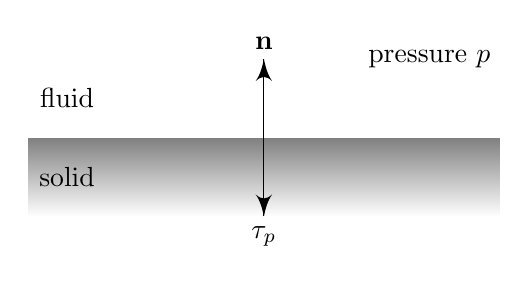
\begin{tikzpicture}
    \fill [gray, path fading=south] (0, 0) rectangle (6, -1);
    \draw [->] (3, 0) -- +(0, 1) node [above] {$\mathbf{n}$};
    \draw [->] (3, 0) -- +(0, -1) node [below] {$\tau_p$};
    \node at (0.5, -0.5) {solid};
    \node at (0.5, 0.5) {fluid};
    \node at (6, 1) [left] {pressure $p$};
  \end{tikzpicture}
\end{center}
Suppose we have a fluid with pressure $p$ acting on a surface with unit normal $\mathbf{n}$, pointing \emph{into} the fluid.

\begin{defi}[Normal stress]
  The \emph{normal stress} is
  \[
    \tau_p = -p\mathbf{n}.
  \]
\end{defi}
Gradients in pressure produce a force. For example, suppose we have a pipe, with the pump on the left:
\begin{center}
  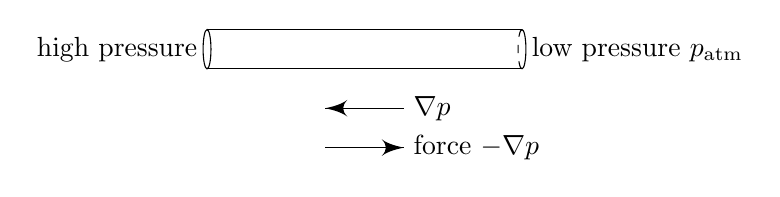
\begin{tikzpicture}
    \draw (0, 0) -- +(4, 0);
    \node at (0, 0.25) [left] {high pressure};
    \node at (4, 0.25) [right] {low pressure $p_{\mathrm{atm}}$};
    \draw (0, 0.5) -- +(4, 0);
    \draw [->] (2.5, -0.5) node [right] {$\nabla p$} -- +(-1, 0);
    \draw [->] (1.5, -1) -- +(1, 0) node [right] {force $-\nabla p$};
    \draw (0, 0.25) ellipse (0.05 and 0.25);
    \draw [dashed] (4, 0) arc (270:90:0.05 and 0.25);
    \draw (4, 0) arc (270:450:0.05 and 0.25);
  \end{tikzpicture}
\end{center}
This gives a \emph{body force} that drives the water from left to right.

\subsubsection{Tangential stress}
Consider two infinite planes with fluids in between. We keep the bottom plane at rest, and move the top plate with velocity $U$.
\begin{center}
  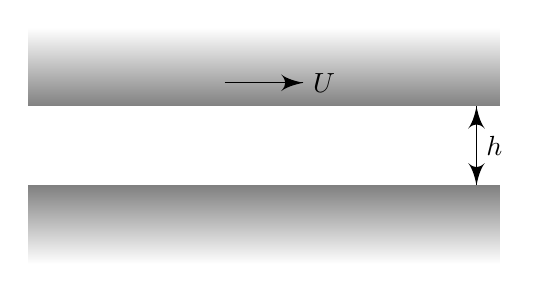
\begin{tikzpicture}
    \fill [gray, path fading=south] (0, 0) rectangle (6, -1);
    \fill [gray, path fading=north] (0, 1) rectangle (6, 2);
    \draw [->] (2.5, 1.3) -- +(1, 0) node [right] {$U$};

    \draw [<->] (5.7, 0) -- +(0, 1) node [right, pos=0.5] {$h$};
  \end{tikzpicture}
\end{center}

\begin{defi}[Tangential stress]
  The \emph{tangential stress} $\tau_s$ is the force (per unit area) required to move the top plate at speed $U$.
\end{defi}

Experimentally, we find the following.
\begin{law}
  For a Newtonian fluid, we have
  \[
    \tau_s \propto \frac{U}{h}.
  \]
\end{law}

\begin{defi}[Dynamic viscosity]
  The \emph{dynamic viscosity} $\mu$ of the fluid is the constant of proportionality in
  \[
    \tau_s = \mu \frac{U}{h}.
  \]
\end{defi}

We find the dimensions of these quantities as
\begin{align*}
  [\tau_s] &= ML^{-1} T^{-2}\\
  \left[\frac{U}{h}\right] &= T^{-1}\\
  [\mu] &= ML^{-1} T^{-1}.
\end{align*}
In SI units, $\mu$ has units $\SI{}{\kilo\gram\per\meter\per\second}$.

We have not yet said what the fluid in the middle does. It turns out this is simple: at the bottom, the fluid is constant, and at the top, the fluid moves with velocity $U$. In between, the speed varies linearly.
\begin{center} % put axes in gray
  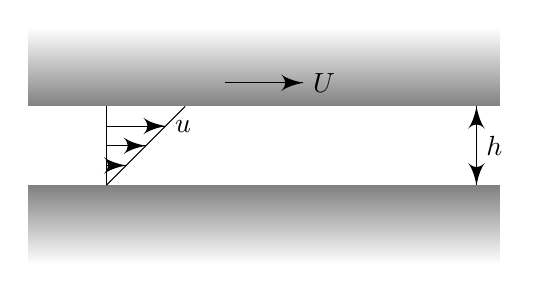
\begin{tikzpicture}
    \fill [gray, path fading=south] (0, 0) rectangle (6, -1);
    \fill [gray, path fading=north] (0, 1) rectangle (6, 2);
    \draw [->] (2.5, 1.3) -- +(1, 0) node [right] {$U$};

    \draw [<->] (5.7, 0) -- +(0, 1) node [right, pos=0.5] {$h$};

    \draw (1, 0) -- (1, 1);
    \draw (1, 0) -- (2, 1);
    \foreach \x in {0,0.25,0.5,0.75} {
      \draw [->] (1, \x) -- (1 + \x, \x);
    }
    \node at (1.75, 0.75) [right] {$u$};
  \end{tikzpicture}
\end{center}
We will derive this formally later.

For a general flow, let $u_T(\mathbf{x})$ be the velocity of the fluid at position $\mathbf{x}$. Then the tangential stress is
\[
  \tau_s = \mu \frac{\partial u_T(\mathbf{x})}{\partial \mathbf{n}},
\]
and is in the direction of the tangential component of velocity. Again, the normal vector $\mathbf{n}$ points \emph{into} the fluid.

\subsection{Steady parallel viscous flow}
We first explain what the words in the title mean. Steady means there is no change in time, ie. there is no acceleration. In other words, all forces balance.

``Parallel'' means the fluid only flows in one dimension, and only depends on the direction perpendicular to the plane. So the velocity can be written as
\[
  \mathbf{u} = (u(y), 0, 0).
\]
We can draw a flow profile as follows:
\begin{center}
  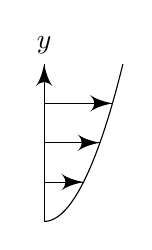
\begin{tikzpicture}
    \draw (0, 0) parabola (1, 2);
    \foreach \x in {0,0.25,0.5,0.75} {
      \pgfmathsetmacro\len{sqrt(\x)}
      \draw [->] (0, 2*\x) -- +(\len, 0);
    }
    \draw [->] (0, 0) -- (0, 2) node [above] {$y$};
  \end{tikzpicture}
\end{center}
We consider a small box in the fluid:
\begin{center}
  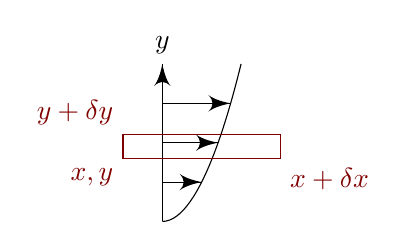
\begin{tikzpicture}
    \draw (0, 0) parabola (1, 2);
    \foreach \x in {0,0.25,0.5,0.75} {
      \pgfmathsetmacro\len{sqrt(\x)}
      \draw [->] (0, 2*\x) -- +(\len, 0);
    }
    \draw [->] (0, 0) -- (0, 2) node [above] {$y$};
    \draw [mred] (-0.5, 0.8) node [anchor = north east] {$x, y$} -- +(2, 0) node [anchor = north west] {$x + \delta x$} -- +(2, 0.3) -- +(0, 0.3) node [anchor = south east] {$y + \delta y$} -- cycle;
  \end{tikzpicture}
\end{center}
We know that this block of fluid moves in the $x$ direction without acceleration. So the total forces of the surrounding environment on the box should vanish.

We first consider the $x$ direction. There are normal stresses at the sides, and tangential stresses at the top and bottom. The sum of forces in the $x$-direction (per unit transverse width) gives
\[
  p(x) \delta y - p(x + \delta x) \delta y + \tau_s(y + \delta y) \delta x + \tau_s(y) \delta x = 0.
\]
By the definition of $\tau_s$, we can write
\[
  \tau_s(y + \delta y) = \mu \frac{\partial u}{\partial y}(y + \delta y),\quad \tau_s (y) = -\mu \frac{\partial u}{\partial y}(y),
\]
where the different signs come from the different normals (for a normal pointing downwards, $\frac{\partial}{\partial \mathbf{n}} = \frac{\partial}{\partial -y}$).

Dividing by $\delta x \delta y$ and take the limit as $\delta x, \delta y \to 0$, we end up with the equation of motion
\[
  -\frac{\partial p}{\partial x} + \mu \frac{\partial^2 u}{\partial y^2} = 0.\tag{1.2a}
\]
Looking at the $y$ direction, we find
\[
  -\frac{\partial p}{\partial y} = 0.\tag{1.2b}
\]
In the second equation, we keep the negative sign for consistency, but obviously in this case it is not necessary.

This is the simplest possible case. We can extend this a bit by allowing, say, non-steady flows, For unsteady parallel viscous flows
\[
  \mathbf{u} = (U(u, t), 0, 0)
\]
of an (incompressible) fluid acted on by a body force (per unit volume) $(f_x, f_y, 0)$, we obtain the equations
\begin{align*}
  \rho\frac{\partial u}{\partial t} &= -\frac{\partial p}{\partial x} + \mu \frac{\partial^2 u}{\partial y^2} + f_x\tag{1.3a}\\
  0 &=-\frac{\partial p}{\partial y} + f_y.\tag{1.3b}
\end{align*}
You will derive these in example sheet 1. Here $\rho$ is the density, ie. the mass per unit volume. For air, it is approximately $\SI{1}{\kilo\gram\per\meter\cubed}$, and for water, it is approximately $\SI{1000}{\kilo\gram\per\meter\cubed}$.

Here we said that the fluid is incompressible, which means it cannot be compressed (duh). We will give a form definition later. In general, though, fluids are not compressible. For example, sound waves are exactly waves of compression in air, and cannot exist if air is incompressible. Alternatively, we say that sound travels at an infinite speed.

Hence, compressibility matters mostly when we are travelling near the speed of sound. If we are moving in low speeds, we can just pretend the fluid is indeed incompressible.

\subsection{Boundary conditions for viscous fluids}
Experimentally, we found (down to 2 molecular diameters for water, approximately $\SI{6}{\angstrom}$) that Newtonian fluids satisfy one of the following two boundary conditions:
\begin{enumerate}
  \item \emph{No-slip condition}: at the boundary, the tangential component of the fluid velocity equals the tangential velocity of boundary. In particular, if the boundary is stable, the tangential component of the fluid velocity is zero. This means fluids stick to surfaces.
    \[
      u_T = 0.\tag{1.5}
    \]
  \item \emph{Stress condition}: alternatively, a tangential stress $\tau$ is imposed on the fluid. In this case,
    \[
      -\mu \frac{\partial u_T}{\partial n} = \tau.\tag{1.5}
    \]
\end{enumerate}

We are going to look at some examples.
\subsection{Couette flow}
This is the flow driven by the motion of a boundary.
\begin{center}
  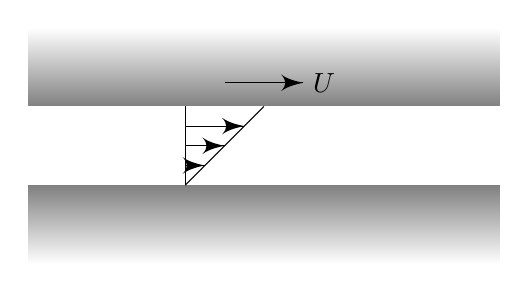
\begin{tikzpicture}
    \fill [gray, path fading=south] (0, 0) rectangle (6, -1);
    \fill [gray, path fading=north] (0, 1) rectangle (6, 2);
    \draw [->] (2.5, 1.3) -- +(1, 0) node [right] {$U$};

    \draw (2, 0) -- (2, 1);
    \draw (2, 0) -- (3, 1);

    \foreach \x in {0.25,0.5,0.75} {
      \draw [->] (2, \x) -- +(\x, 0);
    }
  \end{tikzpicture}
\end{center}
We assume that this is a stead flow, and there is no pressure gradient. So our equations give
\[
  \frac{\partial^2 u}{\partial y^2} = 0.
\]
Moreover, we have the boundary condition of $u = 0$ on $y = 0$; $u = U$ on $y = h$. The solution is thus
\[
  u = \frac{U y}{h}.
\]
\subsection{Pouseuille flow}
This is a flow driven by a pressure gradient between stationary boundaries. Again we have two boundaries
\begin{center}
  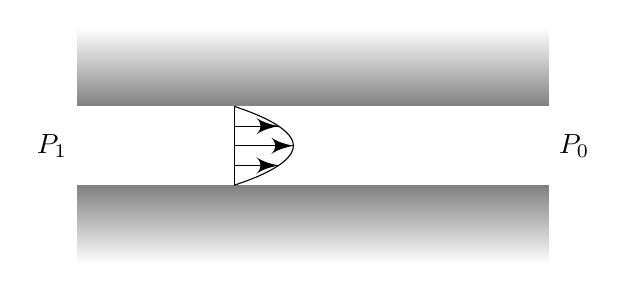
\begin{tikzpicture}
    \fill [gray, path fading=south] (0, 0) rectangle (6, -1);
    \fill [gray, path fading=north] (0, 1) rectangle (6, 2);

    \node [left] at (0, 0.5) {$P_1$};
    \node [right] at (6, 0.5) {$P_0$};

    \foreach \x in {0.25,0.5,0.75} {
      \pgfmathsetmacro\len{\x * (1 - \x)}
      \draw [->] (2, \x) -- +(3 * \len, 0);
    };
    \draw [rotate=270, yscale=-1, shift={(-3,-3)}] (2.5, 0.25) parabola (2, 1);% magic
    \draw [rotate=90, shift={(-2,-3)}] (2.5, 0.25) parabola (2, 1);
    \draw (2, 0) -- (2, 1);
  \end{tikzpicture}
\end{center}
We have a high pressure $P_1$ on the left, and a low pressure $P_0 < P_1$ on the right. We solve this problem again, but we will also include gravity. So the equations of motion become
\begin{align*}
  -\frac{\partial p}{\partial x} + \mu\frac{\partial^2 u}{\partial y^2} &= 0\\
  -\frac{\partial p}{\partial y} - g\rho &= 0
\end{align*}
The boundary conditions are $u = 0$ at $y = 0, h$. The second equation implies
\[
  p =- g\rho y + f(x)
\]
for some function $f$. Substituting into the first gives
\[
  \mu\frac{\partial^2 u}{\partial y^2} = f'(x).
\]
The left is a function of $y$ only, while the right depends only on $x$. So both must be constant, say $G$. Using the boundary conditions, we get
\[
  \mu\frac{\partial^2 u}{\partial y^2} = f'(x) = G = \frac{P_1 - P_0}{L},
\]
where $L$ is the length of the tube. Then we find
\[
  u = \frac{G}{2 \mu} y(h - y).
\]
Here the velocity is the greatest at the middle, where $y = \frac{h}{2}$.

Since the equations of motion are linear, if we have both a moving boundary and a pressure gradient, we can just add the tow solutions up.

\subsection{Derived properties of a flow}
We're going to look at some properties of these flows. One thing we want to know is how much of stuff is being transported.

\subsubsection{Volume flux}
\begin{defi}[Volume flux]
  The \emph{volume flux} is the volume of fluid traversing a cross-section per unit time. This is given by
  \[
    q = \int_0^h u(y) \;\d y
  \]
  per unit transverse width.
\end{defi}
We can calculate this immediately for the two flows.

\begin{eg}
  For the Couette flow, we have
  \[
    q = \int_0^h \frac{Uy}{h}\;\d y = \frac{Uh}{2}.
  \]
  For the Pouseuille flow, we have
  \[
    q = \int_0^h \frac{G}{2\mu} y (h - y)\;\d y = \frac{Gh^3}{12 \mu}.
  \]
\end{eg}

\subsubsection{Vorticity}
\begin{defi}[Vorticity]
  The \emph{vorticity} is defined by
  \[
    \boldsymbol\omega = \nabla \times \mathbf{u}.
  \]
\end{defi}
In our case, since we have
\[
  \mathbf{u} = (u(y, t), 0, 0),
\]
we have
\[
  \boldsymbol\omega = \left(0, 0, -\frac{\partial u}{\partial y}\right).
\]
\begin{eg}
  For the case of the Couette flow, the vorticity is $\boldsymbol\omega = \left(0, 0, -\frac{U}{h}\right)$. This is a constant, ie. the vorticity is uniform.
  \begin{center}
    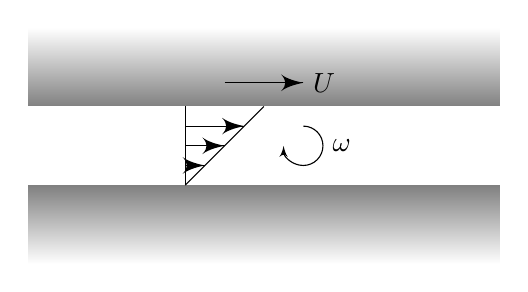
\begin{tikzpicture}
      \fill [gray, path fading=south] (0, 0) rectangle (6, -1);
      \fill [gray, path fading=north] (0, 1) rectangle (6, 2);
      \draw [->] (2.5, 1.3) -- +(1, 0) node [right] {$U$};

      \draw (2, 0) -- (2, 1);
      \draw (2, 0) -- (3, 1);

      \foreach \x in {0.25,0.5,0.75} {
        \draw [->] (2, \x) -- +(\x, 0);
      }
      \draw [-latex'] (3.5, 0.75) arc(90:-180:0.25);
      \node at (3.75, 0.5) [right] {$\omega$};
    \end{tikzpicture}
  \end{center}
  For the case of the Pouseuille flow, we have
  \[
    \boldsymbol\omega = \left(0, 0, \frac{G}{\mu}\left(y - \frac{h}{2}\right)\right).
  \]
\end{eg}
\begin{center}
  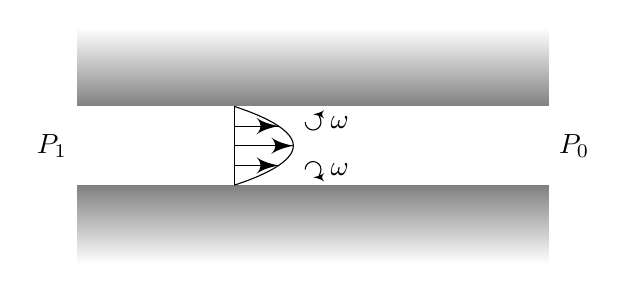
\begin{tikzpicture}
    \fill [gray, path fading=south] (0, 0) rectangle (6, -1);
    \fill [gray, path fading=north] (0, 1) rectangle (6, 2);

    \node [left] at (0, 0.5) {$P_1$};
    \node [right] at (6, 0.5) {$P_0$};

    \foreach \x in {0.25,0.5,0.75} {
      \pgfmathsetmacro\len{\x * (1 - \x)}
      \draw [->] (2, \x) -- +(3 * \len, 0);
    };
    \draw [rotate=270, yscale=-1, shift={(-3,-3)}] (2.5, 0.25) parabola (2, 1);% magic
    \draw [rotate=90, shift={(-2,-3)}] (2.5, 0.25) parabola (2, 1);
    \draw (2, 0) -- (2, 1);

    \draw [-latex'] (2.9, 0.2) arc(180:-90:0.1);
    \node at (3.1, 0.2) [right] {$\omega$};

    \draw [-latex'] (2.9, 0.8) arc(-180:90:0.1);
    \node at (3.1, 0.8) [right] {$\omega$};
  \end{tikzpicture}
\end{center}

\subsubsection{Surface stress}
Recall that $\tau_s$ is the tangential force per unit area exerted by the fluid on the surface, given by
\[
  \tau_s = \mu \frac{\partial u}{\partial \mathbf{n}},
\]
with $\mathbf{n}$ pointing into the fluid.

\begin{eg}
For the Couette flow, we have
\[
  \tau_s =
  \begin{cases}
    \mu \frac{U}{h} & y = 0\\
    -\mu \frac{U}{h} & y = h
  \end{cases}
\]
We see that at $y = 0$, the stress is positive, and pulls the surface forward. At $y = h$, it is negative, and the surface is pulled backwards.

For the Pouseuille flow, we have
\[
  \tau_s =
  \begin{cases}
    \frac{Gh}{2} & y = 0\\
    \frac{Gh}{2} & y = h\\
  \end{cases}
\]
Both surfaces are pulled forward, and this is independent of the viscosity. This makes sense since the force on the surface is given by the pressure gradient, which is independent of the fluid.
\end{eg}
\subsection{Gravity-driven flow down a slope}
\begin{center}
  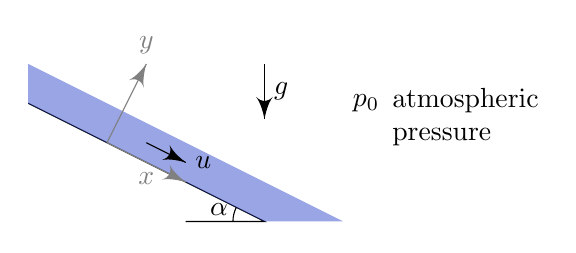
\begin{tikzpicture}
    \draw (0, 1.5) -- (3, 0) -- (2, 0);
    \fill [mblue, opacity=0.5] (0, 1.5) -- (3, 0) -- (4, 0) -- (0, 2) -- cycle;

    \draw [gray, ->] (1, 1) -- +(0.5, 1) node [above] {$y$};
    \draw [gray, ->] (1, 1) -- +(1, -0.5) node [below, pos=0.5] {$x$};
    \draw [->] (3, 2) -- +(0, -0.7) node [pos=0.5, right] {$g$};
    \draw [->] (1.5, 1) -- (2, 0.75) node [right] {$u$};
    \node [right] at (4, 1.5) {$p_0$};
    \node [right, align=left] at (4.5, 1.33) {atmospheric\\ pressure};
    \draw (2.6, 0) arc(180:153.4349:0.4);
    \node [left] at (2.66, 0.15) {$\alpha$};
  \end{tikzpicture}
\end{center}
Here there is just atmosphere above the fluid, and we assume the fluid flow is steady, ie. $u$ is merely a function of $y$. We further assume that the atmospheric pressure does not vary over the vertical extent of the flow. This is a very good approximation because $\rho_{\mathrm{air}} \ll \rho_{\mathrm{liq}}$.

Similarly, we assume $\mu_{\mathrm{air}} \ll \mu_{\mathrm{liq}}$. So the air exerts no significant tangential stress. This is known as a free surface.

We first solve the $y$ momentum equation. The force in the $y$ direction is $-g \rho \cos \alpha$. Hence the equation is
\[
  \frac{\partial p}{\partial y} = - gp \cos \alpha.
\]
Using the fact that $p = p_0$ at the top boundary, we get
\[
  p = p_0 - g\rho \cos \alpha (y - h).
\]
In particular, $p$ is independent of $x$. In the $x$ component, we get
\[
  \mu \frac{\partial^2 u}{\partial y^2} = - g\rho \sin \alpha.
\]
The no slip condition gives $u = 0$ when $y = 0$. The other condition is that there is no stress at $y = h$. So we get $\frac{\partial u}{\partial y} = 0$ when $y = h$.

The solution is thus
\[
  u = \frac{g\rho\sin \alpha}{2 \mu} y(2h - y).
\]
This is a bit like the Poiseuille flow, with $\frac{gp \sin \alpha}{2\mu}$ as the pressure gradient. But instead of going to zero at $y = h$, we get to zero at $y = 2h$ instead. So this is half a Poiseuille flow. % diagram

It is an exercise for the reader to calculate the volume flux $q$.

 % can insert profile
\subsection{Unsteady parallel viscous flow}
Consider fluid initially at rest in $y > 0$, resting on a flat surface.
\begin{center}
  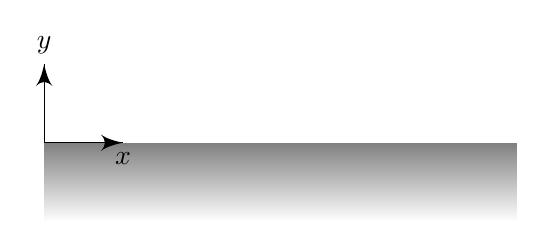
\begin{tikzpicture}
    \fill [gray, path fading=south] (0, 0) rectangle (6, -1);
    \draw [->] (0, 0) -- (0, 1) node [above] {$y$};
    \draw [->] (0, 0) -- (1 , 0) node [below] {$x$};
  \end{tikzpicture}
\end{center}
At time $t = 0$, the boundary $y = 0$ starts to move at constant speed $U$. There is no force and no pressure gradient.

We use the $x$-momentum equation to get
\[
  \frac{\partial u}{\partial t} = \nu \frac{\partial^2 u}{\partial y^2},
\]
where $\nu = \frac{\mu}{\rho}$. This is clearly the diffusion equation, with the diffusivity $\nu$. We can view this as the diffusion coefficient for motion/momentum/vorticity.
\begin{defi}[Kinematic viscosity]
  The \emph{kinematic viscosity} is
  \[
    \nu = \frac{\mu}{\rho}.
  \]
\end{defi}
The boundary conditions are $u = 0$ for $t = 0$ and $u \to 0$ as $y \to \infty$ for all $t$. The other boundary condition is obviously $u = U$ when $y = 0$, for $t > 0$.

You should have learnt how to solve this in, say, IB Methods. We will approach this differently here.
\subsubsection{Dimensional analysis}
We want to do some dimensional analysis. We are already provided with a velocity $U$. We let $T$ be our time scale. We would like to know how fast the movement of fluid propagates up the $y$ axis. We note that in this case, we don't really have an extrinsic length scale --- in the case where we have two boundaries, the distance between them is a natural length scale to compare with, but here the fluid is infinitely thick. So we need to come up with a characteristic intrinsic length scale somewhat arbitrarily. For example, at any time $T$, we can let $\delta$ be the amount of fluid that has reached a speed of at least $\frac{U}{10}$.

Instead of trying to figure out the dimensions of, say, $\nu$ and trying to match them, we just replace terms in the differential equation with these quantities of the right dimension, since we know our differential equation is dimensionally correct. So we obtain
\[
  \frac{U}{T} \sim \nu \frac{U}{\delta^2}.
\]
Since the $U$ cancels out, we get
\[
  \delta \sim \sqrt{\nu T}.
\]
We can figure out approximately how big this is. For water, we have $\nu_{\mathrm{water}} \approx \SI{10e-6}{\meter\squared\per\second}$. For air, we have $\nu_{\mathrm{air}} \approx \SI{10e-5}{\meter\squared\per\second}$. These are, in general, very tiny.
\subsubsection{Similarity solution}
We now solve the problem properly. In an infinite domain with no extrinsic length scale, the diffusion equation admits a similarity solution. We write
\[
  u(y, t) = U f(\eta),
\]
where $f(\eta)$ is a dimensionless function of the dimensionless variable $\eta$. To make $y$ dimensionless, we define
\[
  \eta = \frac{y}{\delta} = \frac{y}{\sqrt{\nu t}}.
\]
We substitute this form of the solution into the differential equation. Then we get
\[
  -\frac{1}{2} \eta f'(\eta) = f''(\eta),
\]
with boundary condition $f = 1$ on $\eta = 0$. Then the solution is by definition
\[
  f = \erfc \left(\frac{\eta}{2}\right).
\]
Hence
\[
  u = U \erfc \left(\frac{y}{2\sqrt{\eta t}}\right).
\]
\begin{center}
  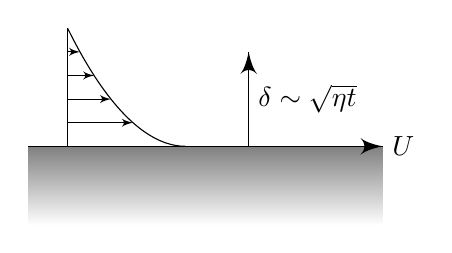
\begin{tikzpicture}
    \fill [gray, path fading=south] (0.5, 0) rectangle (5, -1);
    \draw [->] (0.5, 0) -- (5, 0) node [right] {$U$};
    \draw [->] (3.3, 0) -- +(0, 1.2) node [right, pos=0.5] {$\delta \sim \sqrt{\eta t}$};

    \draw (1, 0) -- (1, 1.5);
    \draw (2.5, 0) parabola (1, 1.5);
    \foreach \y in {0.3,0.6,0.9,1.2} {
      \pgfmathsetmacro\x{1.5 - sqrt(1.5 * \y)};
      \draw [-latex'] (1, \y) -- +(\x, 0);
    }
  \end{tikzpicture}
\end{center}

\subsubsection{Kinematic and dynamic viscosities}
Here we note the viscosities of some common fluids
\begin{center}
  \begin{tabular}{cccc}
    \toprule
    & $\mu(\SI{}{\kilo\gram\per\meter\per\second})$ & $\rho(\SI{}{\kilo\gram\per\meter\cubed})$ & $\nu(\SI{}{\meter\squared\per\second})$\\
    \midrule
    water & $10^{-3}$ & $10^3$ & $10^{-6}$\\
    air & $10^{-5}$ & $1$ & $10^{-5}$\\
    \bottomrule
  \end{tabular}
\end{center}
We can compute the tangential stress of the fluid in the above case to be
\[
  \tau_s \mu\frac{\partial u}{\partial y} = \left.\mu \frac{U}{\sqrt{\nu t}} \left(\frac{2}{\sqrt{\pi}}\right) e^{-y^{2}}\right|_{y = 0} = \frac{\mu U}{\sqrt{\pi \nu t}}.
\]
For comparison, we find that $\frac{\mu}{\sqrt{\nu}}$ is $1$ for water and $10^{-3}$ for air.

This is significant in, say, the motion of ocean current. When the wind blows, it causes the water in the ocean to move along with it. This is done in a way such that the surface tension between the two fluids match at the boundary. Hence we see that even if the air blows really quickly, the resultant ocean current is much smaller, say a hundredth to a thousandth of it.

\section{Kinematics}
\subsection{Material time derivative}
In this picture, in order to study fluid motion, we mark (with, say, a dye) a fluid particle, and follow its trajectory. This is a very natural thing to do. For example, if we see smoke coming out of a chimney, we follow the smoke and see how it goes. The problem with this is that trajectories can cross, and this makes writing down differential equations difficult.
\begin{center}
  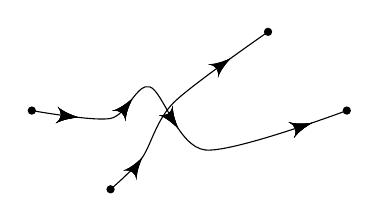
\begin{tikzpicture}
    \node [circ] at (0, 0) {};
    \node [circ] at (4, 0) {};
    \draw [->-=0.13, ->-=0.3, ->-=0.5, ->-=0.9] plot [smooth] coordinates {(0, 0) (1, -0.1) (1.5, 0.3) (2.2, -0.5) (4, 0)};

    \node [circ] at (1, -1) {};
    \node [circ] at (3, 1) {};

    \draw [->-=0.2, ->-=0.8] plot [smooth] coordinates {(1, -1) (1.4, -0.6) (1.8, 0.1) (3, 1)};
  \end{tikzpicture}
\end{center}
There is an alternative way to do this, known as the Eulerian picture (or lazy person's picture). We sit at one place, and watch the world go by. For example, we stand at the top of a tower and hold an instrument still.

This way, we can formulate equations for observables, such as the velocity $\mathbf{u}(\mathbf{x}, t)$, measured at fixed locations as functions of time $t$.

Let's look at these two pictures, and see how they relate to each other. Consider a time-dependent field $f(\mathbf{x}, t)$. For example, it might be the pressure of the system, or the temperature of the fluid. Consider a path $\mathbf{x}(t)$ through the field, and we want to know how the field varies as we move along the path.

Along the path $\mathbf{x}(t)$, the chain rule gives
\begin{align*}
  \frac{\d f}{\d t}(\mathbf{x}(t), t) &= \frac{\partial f}{\partial x} \frac{\d x}{\d t} + \frac{\partial f}{\partial y}\frac{\d y}{\d t} + \frac{\partial f}{\partial z}\frac{\d z}{\d t} + \frac{\partial f}{\partial t}\\
  &= \nabla f \cdot \dot{\mathbf{x}} + \frac{\partial f}{\partial t}.
\end{align*}
\begin{defi}[Material derivative]
  If $\mathbf{x}(t)$ is the (Lagrangian) path followed by a fluid particle, then necessarily $\dot{\mathbf{x}}(t) = \mathbf{u}$ by definition. In this case, we write
  \[
    \frac{\d f}{\d t} = \frac{\D f}{\D t}.
  \]
  This is the \emph{material derivative}.

  In other words, we have
  \[
    \frac{\D f}{\D t} = \mathbf{u}\cdot \nabla f + \frac{\partial f}{\partial t}.
  \]
\end{defi}
On the left of this equation, we have the \emph{Lagrangian derivative}, which is the change in $f$ as we follow the path. On the right of this equation, the first term is $\frac{\partial f}{\partial t}$, the \emph{Eulerian time derivative}, which is the change at a fixed point. The last term is the \emph{advective derivative}, which is the change due to change in position.

For example, consider a river that gets wider as we go downstream. We know (from, say, experience) that the flow is faster upstream than downstream. If the motion is steady, then the Eulerian time derivative vanishes, but the Lagrangian derivative does not, since as the fluid goes down the stream, the fluid slows down, and there is a spacial variation.

In practice, most of the time, we will use the Eulerian formulation, because this allows us to formulate differential equations.

\subsection{Conservation of mass}
The first equation we want to formulate is the conservation of mass.

We fix an arbitrary region of space $\mathcal{D}$ with boundary $\partial \mathcal{D}$ and outward normal $\mathbf{n}$. We imagine there is some flow through this volume
\begin{center}
  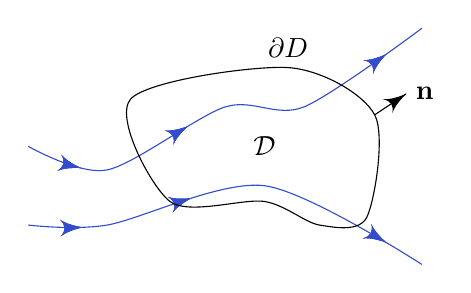
\begin{tikzpicture}
    \draw [mblue, ->-=0.13, ->-=0.4, ->-=0.9] plot [smooth] coordinates {(-3, 0) (-2, -0.3) (-0.5, 0.5) (0.5, 0.5) (2, 1.5)};
    \draw [mblue, ->-=0.13, ->-=0.4, ->-=0.9] plot [smooth] coordinates {(-3, -1) (-2, -1) (0, -0.5) (2, -1.5)};
    \draw plot [smooth cycle] coordinates {(-1.2, -0.7) (0, -0.7) (0.7, -1) (1.3, -0.9) (1.4, 0.4) (0.3, 1) (-1.7, 0.6)};
    \node at (0, 0) {$\mathcal{D}$};
    \node [above] at (0.3, 1) {$\partial D$};
    \draw [->] (1.4, 0.4) -- +(0.4, 0.2666) node [right] {$\mathbf{n}$};
  \end{tikzpicture}
\end{center}
What we want to say is that the change in the mass inside $\mathcal{D}$ is equal to the total flow of fluid through the boundary. We can write this as
\[
  \frac{\d }{\d t}\int_{\mathcal{D}} \rho \;\d V = -\int_{\partial \mathcal{D}} \rho \mathbf{u}\cdot \mathbf{n}\;\d S.
\]
We have the negative sign since we picked the outward normal, and hence the integral measures the outward flow of fluid.

Since the domain is fixed, we can interchange the derivative and the integral on the left; on the right, we can use the divergence theorem to get
\[
  \int_{\mathcal{D}} \left(\frac{\partial \rho}{\partial t} + \nabla \cdot (\rho \mathbf{u})\right) \;\d V = 0.
\]
Since $\mathcal{D}$ was arbitrary, we must have
\[
  \frac{\partial \rho}{\partial t} + \nabla \cdot (\rho \mathbf{u}) = 0
\]
everywhere in space.

This is the general form of a conservation law --- the rate of change of ``stuff'' density plus the divergence of the ``stuff'' flux is constantly zero. We will later formulate a similar result for, say, the momentum.

In the conservation equation, we can expand $\nabla \cdot (\rho \mathbf{u})$ to get
\[
  \frac{\partial \rho}{\partial t} + \mathbf{u}\cdot \nabla \rho + \rho \nabla \cdot \mathbf{u} = 0.
\]
We notice the first term is just the material derivative of $\rho$. So we get
\[
  \frac{\D \rho}{\D t} + \rho \nabla \cdot \mathbf{u} = 0.
\]
\subsection{Incompressible flow}
We have previously handwavily talked about incompressible flows. We now make this notion precise. What exactly happens when we compress a fluid? When we compress mass, in order to conserve mass, we must increase the density. If we don't allow changes in density, then the material derivative $\frac{\D \rho}{\D t}$ must vanish. So we define an incompressible fluid as follows:
\begin{defi}[Incompressible fluid]
  A fluid is \emph{incompressible} if the density of a fluid particle does not change. This implies
  \[
    \frac{\D \rho}{\D t} = 0,
  \]
  and hence
  \[
    \nabla \cdot \mathbf{u} = 0.
  \]
  This is also known as the \emph{continuity equation}.
\end{defi}
For parallel flow, $\mathbf{u} = (u, 0, 0)$. So if the flow is incompressible, we must have $\frac{\partial u}{\partial x} = \nabla \cdot \mathbf{u} = 0$. So we considered $u$ of the form $u = u(y, z, t)$.

Of course, incompressibility is just an approximation. Since we can hear things, everything must be compressible. So what really matters is whether the slow speed is small compared to the speed of sound. If it is relatively small, then incompressibility is a good approximation. In air, the speed of sound is approximately $\SI{340}{\meter\per\second}$. In water, the speed of sound is approximately $\SI{1500}{\meter\per\second}$.

\subsection{Kinematic boundary conditions}
Suppose our system has a boundary. There are two possible cases --- either the boundary is rigid, like a wall, or it moves with the fluid. One important property of the boundary is that fluids are not allowed to pass through them.

To deal with boundaries, we first suppose it has a velocity $\mathbf{U}$ (which may vary with position if the boundary extends through space). We define a local reference frame moving with velocity $\mathbf{U}$, so that in this frame of reference, the boundary is stationary.

In this frame of reference, the fluid has relative velocity
\[
  \mathbf{u}' = \mathbf{u} - \mathbf{U}.
\]
As we mentioned, fluids are not allowed to cross the boundary. Let the normal to the boundary be $\mathbf{n}$, then we must have
\[
  \mathbf{u}' \cdot \mathbf{n} = 0.
\]
In terms of the outside frame, we get
\[
  \mathbf{u}\cdot \mathbf{n} = \mathbf{U} \cdot \mathbf{n}.
\]
This is the condition we have for the boundary.
\subsubsection{Stationary rigid boundary}
If we have a stationary rigid boundary, eg. the wall, then $\mathbf{U} = \mathbf{0}$. So our boundary condition is
\[
  \mathbf{u}\cdot \mathbf{n}= 0.
\]
\subsubsection{Free material boundary}
A good example of a free material body is the surface of a water wave, or interface between two immiscible fluids --- say oil and water.
\begin{center}
  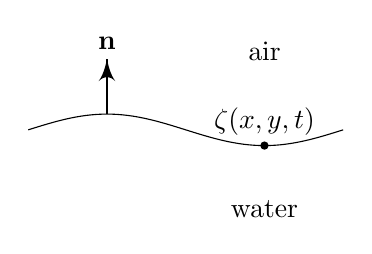
\begin{tikzpicture}
    \draw (0, 0) sin (1, 0.2) cos (2, 0) sin (3, -0.2) cos (4, 0);
    \node at (3, 1) {air};
    \node at (3, -1) {water};

    \draw [->] (1, 0.2) -- +(0, 0.7) node [above] {$\mathbf{n}$};

    \node [circ] at (3, -0.2) {};
    \node [above] at (3, -0.2) {$\zeta(x, y, t)$};
  \end{tikzpicture}
\end{center}
We can define the surface by a function
\[
  z = \zeta(x, y, t).
\]
We can alternatively define the surface as a contour of
\[
  F(x, y, z, t) = z - \zeta(x, y, t).
\]
Then the surface is defined by $F = 0$. By IA vector calculus, the normal is parallel to
\[
  \mathbf{n} \parallel \nabla F = (-\zeta_x, -\zeta_y, 1).
\]
Also, we have
\[
  \mathbf{U} = (0, 0, \zeta_t).
\]
We now let the velocity of the fluid be
\[
  \mathbf{u} = (u, v, w).
\]
Then the boundary condition requires
\[
  \mathbf{u}\cdot \mathbf{n} = \mathbf{U}\cdot \mathbf{n}.
\]
In other words, we have
\[
  -u \zeta_x - v\zeta_y + w = \zeta_t.
\]
So we get
\[
  w = u \zeta_x + v\zeta_y + \zeta_t = \mathbf{u}\cdot \nabla \zeta + \frac{\partial \zeta}{\partial t} = \frac{\D \zeta}{\D t}.
\]
So all the boundary condition says is
\[
  \frac{\D \zeta}{\D t} = w.
\]
Alternatively, since $F$ is a material surface, its material derivative must vanish. So
\[
  \frac{\D F}{\D t} = 0,
\]
and this just gives the same result as above. We will discuss surface waves towards the end of the course, and then come back and use this condition.

\subsection{Streamfunction for incompressible flow}
We suppose our fluid is incompressible, ie.
\[
  \nabla \cdot \mathbf{u} = 0.
\]
By IA Vector Calculus, this implies there is a vector potential $\mathbf{A}$ such that
\begin{defi}[Vector potential]
  A \emph{vector potential} is an $\mathbf{A}$ such that
  \[
    \mathbf{u} = \nabla \times \mathbf{A}.
  \]
\end{defi}

\subsubsection{Two-dimensional flow}
Imagine we are living in the $x, y$ plane, and hence
\[
  \mathbf{u} = (u(x, y, t), v(x, y, t), 0).
\]
(we can also imagine this as a flow that does not depend on the $z$ dimension). Then we can immediately know $\mathbf{A}$ is of the form
\[
  \mathbf{A} = (0, 0, \psi(x, y, t)),
\]
Taking the curl of this, we get
\[
  \mathbf{u} = \left(\frac{\partial \psi}{\partial y}, -\frac{\partial \psi}{\partial x}, 0\right).
\]
\begin{defi}[Streamfunction]
  The $\psi$ such that $\mathbf{A} = (0, 0, \psi)$ is the \emph{streamfunction}.
\end{defi}
This streamfunction is both physically significant, and mathematically convenient, as we will soon see.

We look at some properties of the streamfunction
\subsubsection{Properties of the streamfunction}
This is related to question 7 on the first example sheet.

The first thing we can do is to look at the contours $\psi = c$. These have normal
\[
  \mathbf{n} = \nabla \psi = \left(\psi_x, \psi_y, 0\right).
\]
We immediately see that
\[
  \mathbf{u}\cdot \mathbf{n} = \frac{\partial \psi}{\partial x} \frac{\partial \psi}{\partial y} - \frac{\partial \psi}{\partial y}\frac{\partial \psi}{\partial x} = 0.
\]
So the flow is perpendicular to the normal, ie. tangent to the contours of $\psi$.
\begin{defi}[Streamlines]
  The \emph{streamlines} are the contours of the streamfunction $\psi$.
\end{defi}
This gives an instantaneous picture of flow.

Note that if the flow is \emph{unsteady}, then the streamlines are \emph{not} particle paths.
\begin{eg}
  Consider $\mathbf{u} = (t, 1, 0)$. When $t = 0$, the velocity is purely in the $y$ direction, and the streamlines are also vertical; at $t = 1$, the velocity makes an $45^\circ$ angle with the horizontal, and the streamlines are slanted:
  \begin{center}
    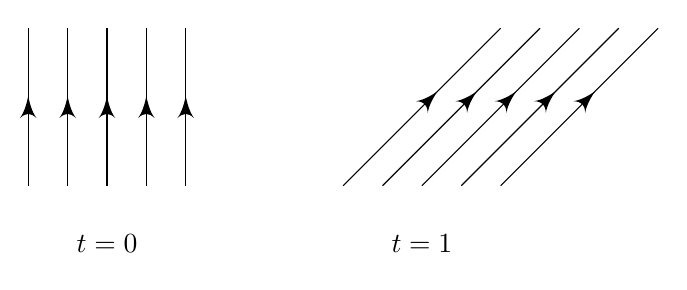
\begin{tikzpicture}
      \draw [->-=0.57] (0, 0) -- +(0, 2);
      \draw [->-=0.57] (0.5, 0) -- +(0, 2);
      \draw [->-=0.57] (1, 0) -- +(0, 2);
      \draw [->-=0.57] (1.5, 0) -- +(0, 2);
      \draw [->-=0.57] (2, 0) -- +(0, 2);

      \node [below] at (1, -0.5) {$t = 0$};

      \begin{scope}[shift={(4, 0)}]
        \draw [->-=0.6] (0, 0) -- +(2, 2);
        \draw [->-=0.6] (0.5, 0) -- +(2, 2);
        \draw [->-=0.6] (1, 0) -- +(2, 2);
        \draw [->-=0.6] (1.5, 0) -- +(2, 2);
        \draw [->-=0.6] (2, 0) -- +(2, 2);

        \node [below] at (1, -0.5) {$t = 1$};
      \end{scope}
    \end{tikzpicture}
  \end{center}
  However, \emph{no} particles will actually follow any of these streamlines. For a particle released at $\mathbf{x}_0 = (x_0, y_0)$. Then we get
  \[
    \dot{x}(t) = u = t,\quad \dot{y} = v = 1.
  \]
  Hence we get
  \[
    x = \frac{1}{2}t^2 + x_0,\quad y = t + y_0.
  \]
  Eliminating $t$, we get that the path is given by
  \[
    (x - x_0) = \frac{1}{2}(y - y_0)^2.
  \]
  So the particle paths are parabolas.
\end{eg}
Typically, we draw streamlines that are ``evenly spaced'', ie. we pick the streamlines $\psi = c_0$, $\psi = c_1$, $\psi c_2$ etc. such that $c_3 - c_2 = c_2 - c_1$.

Then we know the flow is faster where streamlines are closer together:
\begin{center}
  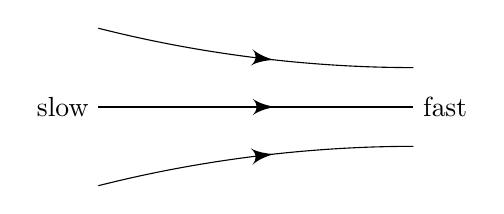
\begin{tikzpicture}
    \draw [-<-=0.44] (4, 0.5) parabola (0, 1);
    \draw [-<-=0.44] (4, 0) -- (0, 0);
    \draw [-<-=0.44] (4, -0.5) parabola (0, -1);

    \node [left] {slow};
    \node [right] at (4, 0) {fast};
  \end{tikzpicture}
\end{center}
This is since the fluid between any two stream lines must be between the stream lines. So if the flow is incompressible, to conserve mass, they mast move faster when the streamlines are closer.

We can also consider the volume flux (per unit length in the $z$-direction), crossing any curve from $\mathbf{x}_0$ to $\mathbf{x}_1$.
\begin{center}
  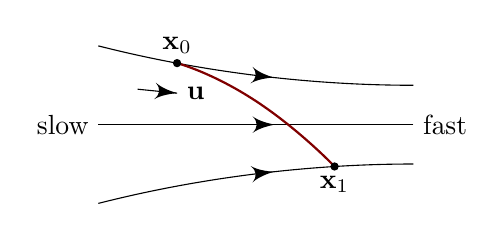
\begin{tikzpicture}
    \draw [-<-=0.44] (4, 0.5) parabola (0, 1);
    \draw [-<-=0.44] (4, 0) -- (0, 0);
    \draw [-<-=0.44] (4, -0.5) parabola (0, -1);

    \draw [mred, thick] plot [smooth, tension=1] coordinates {(1, 0.78125) (2, 0.3) (3, -0.53125)};
    \node [left] {slow};
    \node [right] at (4, 0) {fast};

    \node [circ] at (1, 0.78125) {};
    \node [above] at (1, 0.78125) {$\mathbf{x}_0$};
    \node [circ] at (3, -0.53125) {};
    \node [below] at (3, -0.53125) {$\mathbf{x}_1$};

    \draw [->] (0.5, 0.45) -- (1, 0.4) node [right] {$\mathbf{u}$};

  \end{tikzpicture}
\end{center}
% some flow, path from x_0 to x_1 crossing streamlines, label path as $\Gamma$. Label \mathbf{u} and \mathbf{n}
Then the volume flux is
\[
  q = \int_{\mathbf{x}_0}^{\mathbf{x}_1} \mathbf{u}\cdot \mathbf{n}\;\d \ell.
\]
We see that
\[
  \mathbf{n}\;\d \ell = (-\d y, \d x).
\]
So we can write this as
\[
  q = \int_{\mathbf{x}_0}^{\mathbf{x}_1} -\frac{\partial \psi}{\partial y}\;\d y - \frac{\partial \psi}{\partial x}\;\d x = \psi(\mathbf{x}_0) - \psi(\mathbf{x}_1).
\]
So the flux depends only the difference in the value of $\psi$. Hence, for closer streamlines, to maintain the same volume flux, we need a higher speed.

Also, note that $\psi$ is constant on a stationary rigid boundary, ie. the boundary is a streamline, since the flow is tangential at the boundary. This is a consequence of $\mathbf{u}\cdot \mathbf{n} = 0$. We often choose $\psi = 0$ as our boundary.

\subsubsection{Plane polar coordinates}
We now want to consider two-dimensional flow in plane polars --- we embed these in cylindrical polars $(r, \theta, z)$, with
\[
  \mathbf{u} = \nabla \times (0, 0, \psi) = \frac{1}{r}
  \begin{vmatrix}
    \mathbf{e}_r & r \mathbf{e}_\theta & \mathbf{e}_z\\
    \partial_r & \partial_\theta & \partial_z\\
    0 & 0 & \psi
  \end{vmatrix}
  =\left(r \frac{\partial \psi}{\partial \theta}, -\frac{\partial \psi}{\partial r}, 0\right).
\]
As an exercise, we can verify that $\nabla \cdot \mathbf{u} = 0$. Note that in plane polars,
\[
  \nabla \cdot \mathbf{u} = \frac{1}{r} \frac{\partial}{\partial r} (r \mathbf{u}_r) + \frac{1}{r} \frac{\partial u_\theta}{\partial \theta}.
\]
\section{Dynamics}
\subsection{Navier-Stokes equations}
The Navier-Stokes equation is basically Newton's second law for a fluid particle.
\begin{law}[Navier-Stokes equation]
  \[
    \rho \frac{\D \mathbf{u}}{\D t} = - \nabla p + \mu \nabla^2 \mathbf{u} + \mathbf{f}.
  \]
\end{law}
We will just assume this is true.

This is the general equation for fluid motion. The left hand side is mass times acceleration, and the right is the individual forces --- the pressure gradient, viscosity, and the body forces (per unit volume) respectively.

These are very difficult equations to solve because of non-linearity. For example, in the material derivative, we have the term $\mathbf{u} \cdot \nabla \mathbf{u}$.

There are a few things to note:
\begin{enumerate}
  \item The acceleration of a fluid particle is the Lagrangian material derivative of the velocity.
  \item As we said, the Navier-Stokes equation is per unit volume.
  \item The derivation of the viscous term is complicated, since for each side of the cube, there is one normal direction and two tangential directions. Thus this requires consideration of the \emph{stress tensor}. This is only done in IID Fluid Dynamics.
  \item In a gravitational field, we just have $\mathbf{f} = \mathbf{g}\rho$. This is the only body force we will consider in this course
  \item Note that $\nabla^2 \mathbf{u}$ can be written as
    \[
      \nabla^2 \mathbf{u} = \nabla (\nabla \cdot \mathbf{u}) - \nabla \times (\nabla \times \mathbf{u}).
    \]
    In an incompressible fluid, this reduces to
    \[
      \nabla^2 \mathbf{u} = -\nabla \times (\nabla \times \mathbf{u}) = -\nabla \times \boldsymbol\omega,
    \]
    where $\boldsymbol\omega = \nabla \times \mathbf{u}$ is the vorticity. In Cartesian coordinates, for $\mathbf{u} = (u_x, u_y, u_z)$, we have
    \[
      \nabla^2 \mathbf{u} = (\nabla^2 u_x, \nabla^2 u_y, \nabla^2 u_z),
    \]
    where
    \[
      \nabla^2 = \pd[2]{x} + \pd[2]{y} + \pd[2]{z}.
    \]
  \item The Navier-Stokes equation reduces to the parallel flow equation in the special case of parallel flow, ie. $\mathbf{u} = (u(y, t), 0, 0)$. This verification is left as an exercise for the reader.
\end{enumerate}

\subsection{Hydrostatic pressure}
Hydrostatic pressure is the pressure in a fluid at rest (hence ``hydro'' and ``static''). In other words, $\mathbf{u} = 0$. We done the hydrostatic pressure as $p_H$. Then the Navier-Stokes equation reduces to
\[
  \nabla p_H = \mathbf{f} = \rho \mathbf{g}.
\]
We can integrate this to obtain
\[
  p_h = p \mathbf{g}\cdot \mathbf{x} + p_0,
\]
where $p_0$ is some arbitrary constant. Usually, we have $\mathbf{g} = (0, 0, -g)$. Then
\[
  p_h = p_0 - g \rho z.
\]
In other words, it is just the weight of the fluid above you (per unit area).

\subsubsection{Force on a submerged body in a fluid at rest}
Suppose we have a body $\mathcal{D}$ with boundary $\partial \mathcal{D}$ and outward normal $\mathbf{n}$. Then the force is
\begin{align*}
  \mathbf{F} &= - \int_{\partial \mathcal{D}} p_H \mathbf{n}\cdot dS \\
  &= - \int_\mathcal{D} \nabla p_H \;\d V\\
  &= - \int_{\mathcal{D}} \mathbf{g} \rho \;\d V\\
  &= - \mathbf{g} \int_\mathcal{D} \rho \;\d V\\
  &= - M\mathbf{g},
\end{align*}
where $M$ is the mass of fluid displaced. This is Archimedes' principle.

In particular, if the body is less dense than the fluid, it will float; if the body is denser than the fluid, it will sink; if the density is the same, then it does not move, and we say it is neutrally buoyant.

This is valid only when nothing is moving. So we want to know what happens when things move.

\subsection{Dynamic pressure}
This is what is causing or resulting from fluid flow. For example, in the Poiseuille flow, we have a pressure driving the fluid flow; if we have a flow, this can also create some extra pressure.

In general, we write
\[
  p = p_H + p',
\]
where $p_H$ is the hydrostatic pressure, and $p'$ caused/results from motion.

We substitute this into the Navier-Stokes equation to obtain
\[
  \rho \frac{\D u}{\D t} = -\nabla p' + \mu \nabla^2 \mathbf{u}.
\]
What we usually do is drop the ``prime'', and just look at the deviation from hydrostatic pressure. What this means is that gravity no longer plays a role, and we can ignore gravity in any flow in which the density is constant. Then all fluid particles are neutrally buoyant. This is the case in most of the course, except when we consider motion of water waves, since there is a difference in air density and water density.

\subsection{Reynolds number}
As we mentioned, the Navier-Stokes equation is very difficult to solve. So we want to find some approximations to the equation. We would like to know if we can ignore some terms. For example, if we can neglect the viscous term, then we are left with a first-order equation, not a second-order one.

To do so, we look at the balance of terms, and see if some terms dominate the others. This is done via Reynolds number.

We suppose the flow has a characteristic speed $U$ and an extrinsic length scale $L$, externally imposed by geometry. For example, if we look at the flow between two planes, the characteristic speed can be the maximum (or average) speed of the fluid, and a sensible length scale would be the length between the planes.

Next, we have to define the time scale $T = L/U$. Finally, we suppose pressure \emph{differences} have characteristic magnitude $P$. We are concerned with differences since it is pressure differences that drive the flow.

We are going to take the Navier-Stokes equation, and look at the scales of the terms. Dividing by $\rho$, we get
\[
  \frac{\partial \mathbf{u}}{\partial t} + \mathbf{u}\cdot \nabla \mathbf{u} = -\frac{1}{\rho} \nabla p + \nu \nabla^2 \mathbf{u},
\]
where again $\nu = \frac{\mu}{\rho}$. We are going to estimate the size of these terms. We get
\[
  \frac{U}{(L/U)} \quad\quad U \cdot \frac{U}{L} \quad\quad \frac{1}{\rho} \frac{P}{L} \quad\quad \nu \frac{U}{L^2}.
\]
Dividing by $U^2/L$, we get
\[
  1 \quad\quad 1 \quad\quad \frac{P}{\rho U^2} \quad\quad \frac{\nu}{UL}.
\]
\begin{defi}[Reynolds number]
  The \emph{Reynolds number} is
  \[
    Re = \frac{UL}{\nu},
  \]
  which is a dimensionless number.
\end{defi}
So if $Re$ is very large, then the viscous term is small, and we can probably neglect it. For example, for an aircraft, we have $U \sim 10^4$, $L \sim 10$ and $\nu \sim 10^{-5}$. So the Reynolds number is small, and we can ignore the viscous term. On the other hand, if we have a small slow-moving object in viscous fluid, then $Re$ will be small, and the viscous term is significant.

The Reynolds number $Re$ is a measure of the magnitude of the inertia to viscous terms. The pressure always scales to balance the dominant terms in the equation, so as to impose incompressibility, ie. $\nabla \cdot \mathbf{u} = 0$.

The Reynolds number to a large extent determines the behaviour of a flow. For example, even though lava is very very viscous, on a large scale, the flow of lava is just like the flow of water in a river, since they have comparable Reynolds number.

\begin{defi}[Dynamic similarity]
  Flows with the same geometry and equal Reynolds numbers are said to be dynamically similar.
\end{defi}

\subsubsection{Small Reynolds number (\texorpdfstring{$Re \ll 1$}{Re << 1})}
When $Re \ll 1$, the inertia terms are negligible, and we now have
\[
  P \sim \frac{\rho\nu U}{L} = \frac{\mu U}{L}.
\]
So the pressure balances the sheer stress. We can approximate the Navier-Stokes equation by dropping the term on the left hand side, and write
\[
  0 = -\nabla p + \mu \nabla^2 \mathbf{u},
\]
with the incompressibility condition
\[
  \nabla \cdot \mathbf{u} = 0.
\]
These are known as \emph{Stokes equations}. This is now a linear equation, with four equations and four unknowns (three components of $\mathbf{u}$ and one component of pressure). We find
\[
  \mathbf{u} \propto \nabla p,
\]
and so the velocity is proportional to the pressure gradient.

\subsubsection{Large Reynolds number (\texorpdfstring{$Re \gg 1$}{Re >> 1})}
When $Re \gg 1$, the viscous terms are negligible on extrinsic length scale. Then the pressure scales on the momentum flux,
\[
  P \sim \rho U^2,
\]
and on extrinsic scales, we can approximate Navier-Stokes equations by the \emph{Euler equations}
\begin{align*}
  \rho \frac{\D u}{\D t} &= - \nabla p\\
  \nabla \cdot \mathbf{u} &= 0.
\end{align*}
In this case, the acceleration is proportional to the pressure gradient.

Why do we keep saying ``extrinsic scale''? Note that when we make this approximation, the order of the differential equation drops by $1$. So we can no longer satisfy all boundary conditions. The boundary condition we have to give up is the no-slip condition. So when we make this approximation, we will have to allow the fluid at the boundary to have non-zero velocity.

When is this approximation valid? It is obviously wrong when we are \emph{at} the boundary. If the velocity gradient near the boundary is relatively large, then we quickly get significant non-zero velocity when we move away from boundary, and hence obtain the ``correct'' answer. So we get problems only at the length scale where the viscous and inertia effects are comparable, ie. the \emph{intrinsic} length scale.

\subsubsection{Intrinsic length scale \texorpdfstring{$\delta$}{delta}}
The \emph{intrinsic length scale} $\delta$ is the scale at which the viscous and inertia terms are comparable. Since we need
\[
  U^2 \sim \frac{\nu U}{\delta^2},
\]
we get
\[
  \delta = \frac{\nu}{U}.
\]
Alternatively, we have
\[
  \frac{\delta}{L} = \frac{\nu}{UL} = \frac{1}{Re}.
\]
Thus, for large Reynolds number, the intrinsic length scale, which is the scale in which the viscous and boundary effects matter, is small, and we can ignore them.

For much of the rest of this course, we will ignore viscosity, and consider \emph{inviscid flow}.
\subsection{A case study: stagnation point flow (\texorpdfstring{$\mathbf{u} = \mathbf{0}$}{u = 0})}
There is an exact solution to to the Navier-Stokes equation in the half-plane $y \geq 0$, in which $\mathbf{u} \to (Ex, -E y, 0)$, where $E > 0$ is a constant, as $y \to \infty$, and $\mathbf{u} = \mathbf{0}$ on $y = 0$.
\begin{center}
  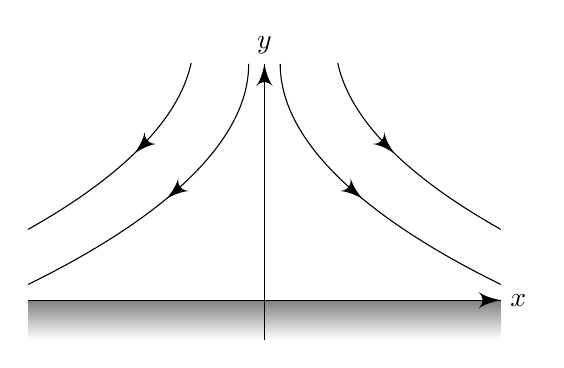
\begin{tikzpicture}
    \fill [gray, path fading=south] (-3, 0) rectangle (3, -0.5);
    \draw [->] (-3, 0) -- (3, 0) node [right] {$x$};
    \draw [->] (0, -0.5) -- (0, 3) node [above] {$y$};

    \draw [->-=0.5, rotate=90](3, 0.2) parabola (0.2, 3);
    \draw [->-=0.5, xscale=-1, rotate=90](3, 0.2) parabola (0.2, 3);

    \clip (-3, 3) rectangle (3, 0);
    \draw [->-=0.5, rotate=90](3.3, 0.9) parabola (0.9, 3);
    \draw [->-=0.5, xscale=-1, rotate=90](3.3, 0.9) parabola (0.9, 3);
  \end{tikzpicture}
\end{center}
The boundary conditions as $y \to \infty$ gives us a picture of what is going on at large $y$, as shown in the diagram, but near the boundary, the velocity has to start to vanish. So we would want to solve the equations to see what happens near the boundary.

Again, this problem does not have any extrinsic length scale. So we can seek a similarity solution of the form
\[
  \mathbf{u} = (u, v, 0) = (Ex g'(\nu), -E \delta g(\eta), 0),
\]
where
\[
  \eta = \frac{y}{\delta}, \quad \delta = \sqrt{\frac{\nu}{E}}.
\]
Hence
\[
  \eta = \sqrt{\frac{E}{\nu}} y.
\]
We want to solve this exactly, and look at the properties of the solution.

First of all, we make sure this is the right similarity solution. We show that $\delta$ has dimensions of length:
\begin{itemize}
  \item The dimension of $E$ is $[E] = T^{-1}$
  \item The dimension of $\nu$ is $[\nu] = L^2 T^{-1}$.
\end{itemize}
Hence
\[
  \left[\frac{E}{\nu}\right] = L^2,
\]
and $\delta$ has dimension $L$. Therefore $\eta = \frac{y}{\delta}$ is dimensionless.

Next, we need to show that this is incompressible. To do this, we simply have to find the streamfunction. It turns out it is given by
\[
  \psi = \sqrt{\nu E} x g(\eta).
\]
We then have
\[
  u = \frac{\partial \psi}{\partial t} = \sqrt{\nu E} x g'(\eta) \frac{1}{\delta} = Ex g'(\eta),
\]
and similarly for the $y$ component. Therefore we must have $\nabla \cdot \mathbf{u} = 0$. Alternatively, we can simply compute $\nabla \cdot \mathbf{u}$ and find it to be zero.

Finally, we look at the Navier-Stokes equations. The $x$ and $y$ components are
\begin{align*}
  u \frac{\partial u}{\partial x} + v \frac{\partial u}{\partial y} &= -\frac{1}{\rho}\frac{\partial p}{\partial x} + \nu \left(\frac{\partial^2 u}{\partial x^2} + \frac{\partial^2 u}{\partial y^2}\right)\\
  u \frac{\partial v}{\partial x} + v \frac{\partial v}{\partial y} &= -\frac{1}{\rho}\frac{\partial p}{\partial y} + \nu \left(\frac{\partial^2 v}{\partial x^2} + \frac{\partial^2 v}{\partial y^2}\right).
\end{align*}
Substituting our expression for $u$ and $v$, we get
\[
  Ex g'E g' - E \delta g E x g'' \frac{1}{\delta} = -\frac{1}{\rho} \frac{\partial p}{\partial x} - \nu E xg''' \frac{1}{\delta^2}.
\]
Some tidying up gives
\[
  E^2 x(g'^2 - gg'') = -\frac{1}{\rho} \frac{\partial p}{\partial x} - E^2 x g'''.
\]
We can do the same thing for the $y$-component, and get
\[
  E\sqrt{\nu E}gg' = -\frac{1}{\rho} \frac{\partial p}{\partial y} - E\sqrt{\nu E}g''.
\]
So we've got two equations for $g$ and $p$. The trick is to take the $y$ derivative of the first, and $x$ derivative of the second, and we can use that to eliminate the $p$ terms. Then we have
\[
  g'g'' - gg''' = g^{(4)}.
\]
So we have a single equation for $g$ that we shall solve.

\subsubsection{Boundary conditions}
We now look at our boundary conditions. The no-slip condition gives $\mathbf{u} = \mathbf{0}$ on $y = 0$. So $g'(0) = g(0) = 0$ when $\eta = 0$.

As as $y \to \infty$, the boundary conditions for $\mathbf{u}$ gives $g'(\eta) \to 1$, $g(\eta) \to \eta$ as $\eta \to \infty$.

All dimensional variables are absorbed into the scaled variables $g$ and $\eta$. So we only have to solve the ODE once. The far field velocity $\mathbf{u} = (Ex, -E y, 0)$ is reached to a very good approximation when
\[
  \eta \lesssim 1,\quad y \lesssim \delta = \frac{\eta}{E}.
\]
\begin{center}
  \begin{tikzpicture}
    \draw [->] (-0.5, 0) -- (5, 0) node [right] {$\eta$};
    \draw [->] (0, -0.5) -- (0, 2.5) node [above] {$g'(\eta)$};
    \draw (0, 0) .. controls (1, 0) and (1, 2) .. (3, 2) -- (5, 2);
    \draw [dashed] (0, 2) -- (3, 2);

    \draw [<->] (0, 1) -- (3, 1) node [pos=0.5, fill=white] {$\delta = O(1)$};
  \end{tikzpicture}
\end{center}

\subsubsection{Overall picture}
We get the horizontal velocity profile as follows:
\begin{center}
  \begin{tikzpicture}
    \draw [->] (-0.5, 0) -- (4, 0) node [right] {$x$};
    \draw [->] (0, -0.5) -- (0, 3) node [above] {$y$};

    \draw (1, 0) arc(270:360:1 and 1.5) -- (2, 3) node [pos=0.5, right] {$Ex$};

    \draw [dashed] (-1, 1.5) -- (4, 1.5);

    \draw [<->] (3, 0) -- (3, 1.5) node [pos=0.5, fill=white] {$\delta$};

    \foreach \x in {0.55, 1.1} {
      \pgfmathsetmacro\y{sqrt(1 - (1 - \x/1.5)^2)};
      \draw [-latex'] (1, \x) -- +(\y, 0);
    }
  \end{tikzpicture}
\end{center}
At the scale $\delta$, we get a Reynolds number of
\[
  Re_\delta = \frac{U\delta}{\nu}\sim O(1).
\]
This is the \emph{boundary layer}. For a larger extrinsic scale $L \gg \delta$, we get
\[
  Re_L = \frac{UL}{2} \gg 1.
\]
\subsubsection{Inviscid approximation}
When interested in flow on scales much larger than $\delta$, we ignore the region $y < \delta$ (since it is small), and we imagine a rigid boundary at $y = \delta$ at which the no-slip condition does not apply.

When $Re_L \gg 1$, we solve the Euler equations, namely
\begin{align*}
  \rho \frac{\D \mathbf{u}}{\D t} &= - \nabla p + \mathbf{f}\\
  \nabla \cdot \mathbf{u} &= 0.
\end{align*}
We still have a boundary condition --- we don't allow fluid to flow \emph{through} the boundary. So we require
\[
  \mathbf{u}\cdot \mathbf{n} = 0\quad\text{at a stationary rigid boundary}.
\]
The no-slip condition is no longer satisfied.

It is an exercise for the reader to show that $\mathbf{u} = (Ex, -Ey, 0)$ satisfies the Euler equations in $y > 0$ with a rigid boundary of $y = 0$, with
\[
  p = p_0 - \frac{1}{2} \rho E^2(x^2 + y^2).
\]
We can plot the curves of constant pressure, as well as the streamlines:
\begin{center}
  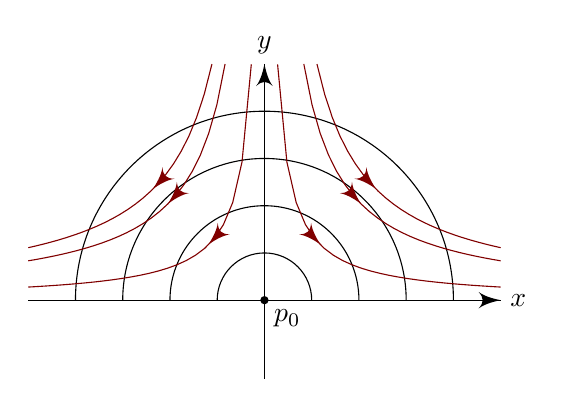
\begin{tikzpicture}
    \draw [->] (-3, 0) -- (3, 0) node [right] {$x$};
    \draw [->] (0, -1) -- (0, 3) node [above] {$y$};
    \foreach \r in {0.6, 1.2, 1.8, 2.4} {
      \draw (\r, 0) arc(0:180:\r);
    }
    \node [circ] {};
    \node [anchor = north west] {$p_0$};

    \draw [mred, ->-=0.5, domain=0.167:3] plot (\x, {0.5/\x});
    \draw [mred, ->-=0.5, domain=0.5:3] plot (\x, {1.5/\x});
    \draw [mred, ->-=0.5, domain=0.667:3] plot (\x, {2/\x});

    \draw [mred, ->-=0.5, domain=0.167:3] plot ({-\x}, {0.5/\x});
    \draw [mred, ->-=0.5, domain=0.5:3] plot ({-\x}, {1.5/\x});
    \draw [mred, ->-=0.5, domain=0.667:3] plot ({-\x}, {2/\x});
  \end{tikzpicture}
\end{center}
As a flow enters from the top, the pressure keeps increases, and this slows down the flow. We say the $y$-pressure gradient is \emph{adverse}. As it moves down and flows sideways, the pressure \emph{pushes} the flow. So the $x$-pressure gradient is \emph{favorable}.

At the origin, the velocity is zero, and this is a \emph{stagnation point}. This is also the point of highest pressure. In general, velocity is high at low pressures and low at high pressures.

\subsection{Momentum equation for inviscid (\texorpdfstring{$\nu = 0$}{nu = 0}) incompressible fluid}
Consider an arbitrary volume $\mathcal{D}$ with boundary $\partial \mathcal{D}$ and outward pointing normal $\mathbf{n}$. The momentum of the fluid in $\mathcal{D}$ can change owing to four things:
\begin{enumerate}
  \item Momentum flux across the boundary $\partial \mathcal{D}$;
  \item Surface pressure forces;
  \item Body forces;
  \item Viscous surface forces.
\end{enumerate}
We will ignore the last one. We can then write the rate of change of the total momentum as
\[
  \frac{\d}{\d t} \int_{\mathcal{D}} p \mathbf{u} \;\d V = -\int_{\partial \mathcal{D}} \rho \mathbf{u} (\mathbf{u}\cdot \mathbf{n}) \;\d S - \int_{\partial \mathcal{D}} p \mathbf{n}\;\d S + \int_{\mathcal{D}} \mathbf{f}\;\d V.
\]
It is helpful to write this in suffix notation. In this case, the equation becomes
\[
  \frac{\d}{\d t} \int_{\mathcal{D}} \rho u_i \;\d V = -\int_{\partial \mathcal{D}} \rho u_i u_j n_j \;\d S - \int_{\partial \mathcal{D}} - p n_i \;\d S + \int_{\mathcal{D}} f_i \;\d V.
\]
Just as in the case of mass conservation, we can use the divergence theorem to write
\[
  \int_{\mathcal{D}} \left(\rho \frac{\partial u_i}{\partial t} + \rho \frac{\partial}{\partial x_j} (u_i u_j)\right)\;\d V = \int_{\mathcal{D}} \left(-\frac{\partial p}{\partial x_i} + f_i\right) \;\d V.
\]
Since $\mathcal{D}$ is arbitrary, we must have
\[
  \rho \frac{\partial u_i}{\partial t} + \rho \frac{\partial u_i}{\partial x_j} + \rho u_i \frac{\partial u_j}{\partial x_j} = -\frac{\partial p}{\partial x_i} + f_i.
\]
The last term on the left is the gradient of $\mathbf{u}$, which vanishes by incompressibility, and the remaining terms is just the material derivative of $\mathbf{u}$. So we get
\begin{prop}[Euler momentum equation]
  \[
    \rho \frac{\D \mathbf{u}}{\d t} = - \nabla p + \mathbf{f}.
  \]
\end{prop}
This is just the equation we get from the Navier-Stokes equation by ignoring the viscous terms. However, we were able to derive this directly from momentum conservation.

For conservative forces, we can write $\mathbf{f} = -\nabla \chi$, where $\chi$ is a scalar potential. For example, gravity can be given by $\mathbf{f} = \rho \mathbf{g} = \nabla (\rho \mathbf{g}\cdot \mathbf{x})$ (for $\rho$ constant). So $\chi = - \rho \mathbf{g}\cdot \mathbf{x} = g \rho z$ if $\mathbf{g} = (0, 0, -g)$.

\subsection{Momentum integral for steady flow}
In the case of a steady flow, $\frac{\partial \mathbf{u}}{\partial t}$ vanishes. Then the momentum equation becomes
\[
  0 = -\int_{\partial \mathcal{D}} \rho \mathbf{u} (\mathbf{u} \cdot \mathbf{n}) \;\d S - \int_{\partial \mathcal{D}}p \mathbf{n} \;\d S - \int_{\mathcal{D}} \nabla \chi \;\d V.
\]
We can then convert this to
\[
  \int_{\partial \mathcal{D}} (\rho \mathbf{u} (\mathbf{u}\cdot \mathbf{n}) + p \mathbf{n} + \chi \mathbf{n}) \;\d S = 0.
\]
\subsection{Bernoulli's equation}
The first thing to notice is we have a vector identity
\[
  \mathbf{u}\times (\nabla \times \mathbf{u}) = \nabla\left(\frac{1}{2}|\mathbf{u}|^2\right) - \mathbf{u}\cdot \nabla \mathbf{u}.
\]
We use this to rewrite the Euler momentum equation as
\[
  \rho \frac{\partial \mathbf{u}}{\partial t} + \rho \nabla \left(\frac{1}{2}|\mathbf{u}|^2\right) - \rho \mathbf{u}\times (\nabla \times \mathbf{u}) = -\nabla p - \nabla \chi.
\]
Dotting with $\mathbf{u}$, the last term on the left vanishes, and we get
\begin{prop}[Bernoulli's equation]
  \[
    \frac{1}{2}\rho \frac{\partial|\mathbf{u}|^2}{\partial t} = -\mathbf{u}\cdot \nabla \left(\frac{1}{2} \rho |\mathbf{u}|^2 + p + \chi\right).
  \]
\end{prop}
In the case where we have a steady flow, we know
\[
  H = \frac{1}{2}\rho |\mathbf{u}|^2 + p + \chi
\]
is constant along streamlines.

Even if the flow is not steady, we can still define the value $H$, and then we can integrate Bernoulli's equation over a volume $\mathcal{D}$ to obtain
\[
  \frac{\d}{\d t}\int_{\mathcal{D}} \frac{1}{2}\rho |\mathbf{u}|^2 \;\d V = -\int_{\partial \mathcal{D}} H \mathbf{u}\cdot \mathbf{n} \;\d S.
\]
So $H$ is the transportable energy of the flow.

\begin{eg}
  Consider a pipe with a constriction. Ignore the vertical pipes for the moment --- they are there just so that we can measure the pressure in the fluid, as we will later see.
  \begin{center}
    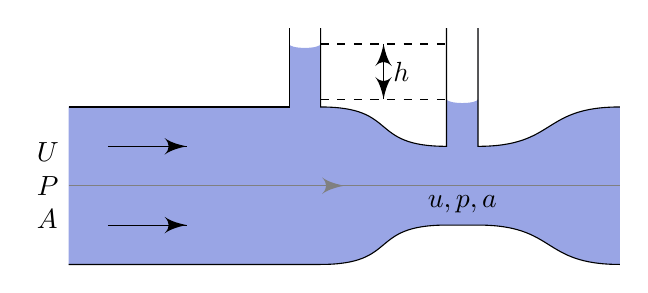
\begin{tikzpicture}
      \fill [mblue, opacity=0.5] (-3, 2) -- (-0.2, 2) -- (-0.2, 2.8) arc(180:360:0.2 and 0.05) -- (0.2, 3) -- (0.2, 2) .. controls (1.2, 2) and (0.8, 1.5) .. (1.8, 1.5) -- (1.8, 2.1) arc(180:360:0.2 and 0.05) -- (2.2, 3) -- (2.2, 1.5) .. controls (3.2, 1.5) and (3, 2) .. (4, 2) -- (4, 0) .. controls (3, 0) and (3.2, 0.5) .. (2.2, 0.5) -- (1.8, 0.5) .. controls (0.8, 0.5) and (1.2, 0) .. (0.2, 0) -- (-3, 0) -- cycle;

      \draw [dashed] (0.2, 2.1) -- (1.8, 2.1);
      \draw [dashed] (0.2, 2.8) -- (1.8, 2.8);

      \draw [<->] (1, 2.1) -- (1, 2.8) node [pos=0.5, right] {$h$};

      \draw (-3, 2) -- (-0.2, 2) -- (-0.2, 3);
      \draw (0.2, 3) -- (0.2, 2) .. controls (1.2, 2) and (0.8, 1.5) .. (1.8, 1.5) -- (1.8, 3);
      \draw (-3, 0) -- (0.2, 0) .. controls (1.2, 0) and (0.8, 0.5) .. (1.8, 0.5) -- (2.2, 0.5) .. controls (3.2, 0.5) and (3, 0) .. (4, 0);
      \draw (2.2, 3) -- (2.2, 1.5) .. controls (3.2, 1.5) and (3, 2) .. (4, 2);

      \draw [gray, ->-=0.5] (-3, 1) -- (4, 1);

      \node [align=left, left] at (-3, 1) {$U$\\$P$\\$A$};
      \node [below] at (2, 1) {$u, p, a$};

      \draw [->] (-2.5, 1.5) -- +(1, 0);
      \draw [->] (-2.5, 0.5) -- +(1, 0);
    \end{tikzpicture}
  \end{center}
  Suppose at the left, we have a uniform speed $U$, area $A$ and pressure $P$. In the middle constricted area, we have speed $u$, area $a$ and pressure $p$.

  By the conservation of mass, we have
  \[
    q = UA = ua.
  \]
  We apply Bernoulli along the central streamline, using the fact that $H$ is constant along streamlines. We can omit the body force $\chi = \rho gy$, since this is the same at both locations. Then we get
  \[
    \frac{1}{2}\rho U^2 + P = \frac{1}{2} \rho u^2 + p.
  \]
  Replacing our $U$ with $q/A$ and $u$ with $q/a$, we obtain
  \[
    \frac{1}{2} \rho \left(\frac{q}{A}\right)^2 + P = \frac{1}{2} \rho \left(\frac{q}{a}\right)^2 + p.
  \]
  Rearranging gives
  \[
    \left(\frac{1}{A^2} - \frac{1}{a^2}\right)q^2 = \frac{2(p - P)}{\rho}.
  \]
  We see there is a difference in pressure due to the difference in area. This is balanced by the difference in heights $h$. Using the $y$-momentum equation, we get
  \[
    \left(\frac{1}{A^2} - \frac{1}{a^2}\right)q^2 = \frac{2(p - P)}{\rho} = -2gh.
  \]
  Then we obtain
  \[
    q = \sqrt{2gh} \frac{Aa}{\sqrt{A^2 - a^2}}.
  \]
  Therefore we can measure $h$ in order to find out the flow rate. This allows us to measure fluid velocity just by creating a constriction and then putting in some pipes.
\end{eg}
Note also that Bernoulli's equation tells us that high velocity goes with low pressure; low pressure goes with high velocity.

\begin{eg}[Force on a fire hose nozzle]
  Suppose we have a fire hose nozzle like this:
  \begin{center}
    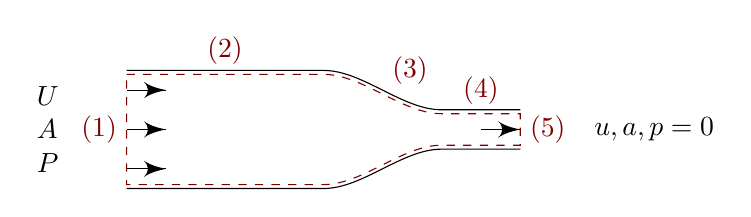
\begin{tikzpicture}
      \draw (-3, 0.75) -- (-0.5, 0.75) .. controls (0, 0.75) and (0.5, 0.25) .. (1, 0.25) -- (2, 0.25);
      \draw (-3, -0.75) -- (-0.5, -0.75) .. controls (0, -0.75) and (0.5, -0.25) .. (1, -0.25) -- (2, -0.25);

      \draw [->] (-3, 0.5) -- +(0.5, 0);
      \draw [->] (-3, 0) -- +(0.5, 0);
      \draw [->] (-3, -0.5) -- +(0.5, 0);

      \draw [->] (1.5, 0) -- +(0.5, 0);

      \draw [mred, dashed] (-3, 0.7) -- (-0.5, 0.7) node [pos=0.5, above] {$(2)$}.. controls (0, 0.7) and (0.5, 0.2) .. (1, 0.2) node [pos=0.5, anchor = south west] {$(3)$} -- (2, 0.2) node [pos=0.5, above] {$(4)$} -- (2, -0.2) node [pos=0.5, right] {$(5)$} -- (1, -0.2) .. controls (0.5, -0.2) and (0, -0.7) .. (-0.5, -0.7) -- (-3, -0.7) -- cycle node [pos=0.5, left] {$(1)$};

      \node [align=left] at (-4, 0) {$U$\\$A$\\$P$};
      \node at (3.7, 0) {$u, a, p = 0$};
    \end{tikzpicture}
  \end{center}
  We consider the steady-flow equation and integrate along the surface indicated above. We integrate each section separately. The end $(1)$ contributes
  \[
    \rho U(-U)A - PA.
  \]
  On $(2)$, everything vanishes. On $(3)$, the first term vanishes since the velocity is parallel to the surface. Then we get a contribution of
  \[
    0 + \int_{\mathrm{nozzle}} p \mathbf{n}\cdot \hat{\mathbf{x}}\;\d S.\tag{3}
  \]
  Similarly, everything in $(4)$ vanishes. Finally, on $(5)$, noting that $p = 0$, we get
  \[
    \rho u^2 a.
  \]
  By the steady flow equation, we know these all sum to zero. Hence, the force on the nozzle is just
  \[
    F = \int_{\mathrm{nozzle}} p\mathbf{n}\cdot \hat{\mathbf{x}}\;\d S = \rho AU^2 - \rho au^2 + PA.
  \]
  We can again apply Bernoulli along a streamline in the middle, which says
  \[
    \frac{1}{2}\rho U^2 + P = \frac{1}{2} \rho u^2.
  \]
  So we can get
  \[
    F = \rho AU^2 - \rho au^2 + \frac{1}{2} \rho A(u^2 - U^2) = \frac{1}{2} \rho\frac{A}{a^2}q^2 \left(1 - \frac{a}{A}\right)^2.
  \]
  Let's now put some numbers in. Suppose $A = (0.1)^2 \pi\SI{}{\meter\squared}$ and $a = (0.05)^2 \pi\SI{}{\meter\squared}$. So we get
  \[
    \frac{A}{a} = 4.
  \]
  A typical fire hose has a flow rate of
  \[
    q = \SI{0.01}{\meter\cubed\per\second}.
  \]
  So we get
  \[
    F = \frac{1}{2} \cdot 1000 \cdot \frac{4}{\pi/40} \cdot 10^{-4} \cdot \left(\frac{3}{4}\right)^2 \approx \SI{14}{N}.
  \]
\end{eg}

\subsection{Linear flows}
We fix our favorite point $\mathbf{x}_0$, and consider the flow in a neighbourhood of $\mathbf{x}_0$. We expand this in a Taylor series:
\begin{align*}
  \mathbf{u}(\mathbf{x}) &= \mathbf{u}(\mathbf{x}_0) + (\mathbf{x} - \mathbf{x}_0) \cdot \nabla \mathbf{u}(\mathbf{x}_0) + \cdots\\
  &= \mathbf{u}_0 + \mathbf{r}\cdot \nabla \mathbf{u}_0,
\end{align*}
with $\mathbf{r} = \mathbf{x} - \mathbf{x}_0$ and $\mathbf{u}_0 = \mathbf{u}(\mathbf{x}_0)$. This is a linear approximation to the flow field. We also write
\[
  \nabla \mathbf{u} = \frac{\partial u_i}{\partial x_j} = E_{ij} + \Omega_{ij} = E + \Omega,
\]
where
\begin{align*}
  E_{ij} &= \frac{1}{2}\left(\frac{\partial u_i}{\partial x_j} + \frac{\partial u_j}{\partial x_i}\right),\\
  \Omega_{ij} &=\frac{1}{2}\left(\frac{\partial u_i}{\partial x_j} - \frac{\partial u_j}{\partial x_i}\right),
\end{align*}
ie. we break $\nabla \mathbf{u}$ up into symmetric and anti-symmetric parts. These different parts have some physical meaning.
\begin{defi}[Vorticity]
  We define the \emph{vorticity} by
  \[
    \boldsymbol\omega = \nabla \times \mathbf{u}.
  \]
\end{defi}
Then we have
\[
  \boldsymbol\omega \times \mathbf{r} = (\nabla \times \mathbf{u}) \times \mathbf{r} = r_j \left(\frac{\partial u_i}{\partial x_j} - \frac{\partial u_j}{\partial x_i}\right) = 2 \Omega_{ij}r_j.
\]
So we can write
\[
  \mathbf{u} = \mathbf{u}_0 + E \mathbf{r} + \frac{1}{2} \boldsymbol\omega \times \mathbf{r}.
\]
The first component is uniform flow; the second is the strain field; and the last is the rotation component.
\begin{center}
  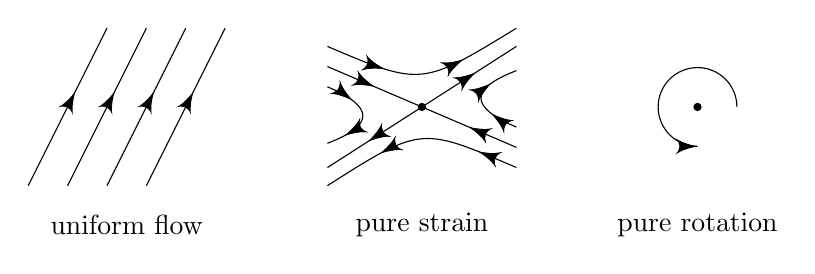
\begin{tikzpicture}
    \foreach \x in {0,0.5,1,1.5} {
      \draw [->-=0.6] (\x, 0) -- +(1, 2);
    }
    \node at (1.25, -0.5) {uniform flow};

    \begin{scope}[shift={(5, 1)}, xscale=0.3, yscale=0.7692]
      \draw [->-=0.785, -<-=0.215] (-4, -1) -- (4, 1);
      \draw [->-=0.25, -<-=0.75] (-4, 0.667) -- (4, -0.667);

      \draw [->- = 0.3, ->- = 0.7] (-4, 1) .. controls (0, 0.333) and (0, 0.35) .. (4, 1.3);
      \draw [-<- = 0.3, -<- = 0.8] (-4, -1.3) .. controls (0, -0.3) and (0, -0.333) .. (4, -1);

      \draw [->- = 0.3, ->- = 0.8] (-4, 0.333) .. controls (-2, 0) and (-2, -0.3) .. (-4, -0.6);
      \draw [->- = 0.3, ->- = 0.7] (4, -0.333) .. controls (2, 0) and (2, 0.3) .. (4, 0.6);
      \node [circ] at (0, 0) {};
    \end{scope}
    \node at (5, -0.5) {pure strain};

    \node [circ] at (8.5, 1) {};

    \draw [->] (9, 1) arc(0:270:0.5);

    \node at (8.5, -0.5) {pure rotation};
  \end{tikzpicture}
\end{center}
Since we have an incompressible fluid, we have $\nabla \cdot \mathbf{u} = 0$. So $E$ has zero trace, ie. if
\[
  E =
  \begin{pmatrix}
    E_1 & 0 & 0\\
    0 & E_2 & 0\\
    0 & 0 & E_3
  \end{pmatrix},
\]
then $E_1 + E_2 + E_3 = 0$. This justifies the picture above.
\end{document}
